\documentclass[onecolumn, compsoc,10pt]{IEEEtran}
\let\labelindent\relax
\usepackage{enumitem}
\input{preamble.tex}  
\def\V{\mathds{V}}
\def\Appendix{Appendix}
%###################################

\newif\iftikzX
\tikzXtrue
\tikzXfalse
%--------------
\def\jobnameX{zero}
%--------------
\newif\ifFIGS
\FIGSfalse 
\FIGStrue
%--------------
\newif\ifdraftQ
\draftQtrue
%\draftQfalse
%--------------
%###################################
\def\TITLE{\enet: Fast Scalable Pandemic Risk Assessment of \infl Strains Circulating In Non-human Hosts}
%\def\TITLE{\LARGE A Biologically Meaningful Sequence Metric\\For Analyzing Evolutionary Changes\\In Novel Pathogens}
%\def\TITLE{Learning  Mutational Patterns At Scale For\\Analysis Of Sequence Divergence\\In Novel Pathogens}
%\def\TITLE{Learning Mutational Patterns at Scale to Analyze Sequence Divergence in Novel Pathogens}

\def\authore{Kevin Wu}
\def\authora{ Jin Li}
\def\authorc{Aaron Esser-Kahn}
\def\authord{Ishanu Chattopadhyay}

\def\addressa{Department of Medicine, University of Chicago, IL, USA}
\def\addressb{Committee on Genetics, Genomics \& Systems Biology, University of Chicago, IL, USA}
\def\addressc{Committee on Quantitative Methods in Social, Behavioral, and Health Sciences, University of Chicago, IL, USA}
\def\addressd{Pritzker School of Molecular Engineering, University of Chicago, Chicago, IL, USA}
\def\addresse{Committee on Immunology, University of Chicago, Chicago, IL, USA}
\newif\ifdraftQ
\draftQtrue
\draftQfalse


%###################################

\title{\LARGE \TITLE}
\author{\sffamily  \fontsize{10}{12}\selectfont   \authore$^{1}$,\authora$^{1}$,  \authorc$^{2,3}$, and \authord$^{1,4,5\bigstar}$\\                                                                
\vspace{10pt}                                                                   

\sffamily  \fontsize{10}{12}\selectfont                                         
$^{1}$\addressa\\   
$^{2}$\addressd\\
$^{3}$\addresse\\
$^{5}$\addressc                                                                 
\vskip 1em                                                                      
$^\bigstar$To whom correspondence should be addressed: e-mail: \texttt{ishanu@uchicago.edu}.}


\def\hcov{SARS-CoV-2\xspace}
\def\RATG13{RaTG13\xspace}
\def\Appendix{Appendix}
\def\qnet{Enet\xspace}
\def\enet{Emergenet\xspace}
\def\erisk{E-risk\xspace}
\def\qdist{E-distance\xspace}
\def\cov{COVID-19\xspace}
\def\infl{Influenza A\xspace}
%\def\infl{IAV\xspace}


\def\E{\mathcal{E}}
\def\dst{x_\star^{t+\delta}}
\def\dsta{x^{t+\delta}}
 
\usepackage{flushend}
\externaldocument[SI-]{SI}
% \externaldocument[EXT-]{exfig}
\newif\iftikzX
\tikzXtrue
\tikzXfalse
\def\Extended{}
\newif\ifFIGS
\FIGSfalse  
\FIGStrue 
 
% Zoonotic risk technology
% FluLeap~\cite{eng2014predicting} is a machine-learning algorithm
% that uses sequence data to identify host tropism: classify influenza
% viruses as either avian or human.
% PREDICT,  a US\$200-million project funded by the
% US Agency for International Development
% (USAID), spent around a decade looking for
% animal viruses. By the time it ended in 2020, it
% had identified 949 new viruses in samples from
% wildlife, livestock and people, in 34 countries

% Zoonotic Risk Technology Enters the Viral Emergence Toolkit
% Grange $\etal$~\cite{grange2021ranking} look for diverse factors,
% but are not strain specific assessments, and identify species
% level risk.

% ~\cite{wille2021accurately} How accurately can we assess zoonotic risk? underscore the
% inherent challanges in assessing  risk from viruses that have not been studied
% well enough.
% genome size may be a useful surrogate in screening for potential zoonotic viruses~\cite{grewelle2020larger}
%
% Among these traits-genomic material, genome segmentation, and replication without nuclear entry-the last is the strongest predictor of cross-species transmission. This finding highlights nuclear entry as a barrier to transmission and suggests that the ability to complete replication in the cytoplasm may prove to be a useful indicator of the threat of cross-species transmission. ~\cite{pulliam2009ability}

  
\tikzexternalenable   
% \pgfplotsset{compat=1.18}
\begin{document}  

\maketitle

{\bf \sffamily \fontsize{10}{12}\selectfont \noindent   
  {\normalfont \itshape Abstract:} Novel \infl  strains emerging into humans from animal reservoirs can cause large antigenic shifts in the circulating strain, and such events are suspected to have triggered numerous  pandemics in the past~\cite{shao2017evolution,mills2004transmissibility,reid2003origin,landolt2007up}, often exacting a devastating toll on human lives. Yet, our current ability to  scalably  evaluate the pandemic potential of   individual strains that do not yet circulate in humans remains limited. In this study, we introduce a computational approach, known as the \enet,  to learn how viable genotypic variations are shaped by  emergent evolutionary constraints using only genomic sequence data of collected strains.    Analyzing    Hemaglutinnin (HA) and Neuraminidase (NA) amino acid sequences from nearly 100,000 unique \infl  strains from public  databases, our proposed algorithm merges machine learning and large deviation theory to  estimate the likelihood of  specific future  mutations, ultimately  yielding the  numerical odds of one parent strain giving rise to a specific descendant via natural evolutionary processes. After validating our model on the problem of forecasting the dominant strain(s) of the upcoming flu season, with \enet-based forecasts significantly outperforming World Health Organization (WHO) recommended flu vaccine compositions almost consistently over the past two decades for  H1N1 and H3N2 subtypes, individually in the Northern and the Southern hemispheres (HA: $34.8\% $ improvement, NA: $12.5\%$ improvement), we assess  the pandemic potential  of novel animal  strains that do not yet circulate in humans. While the state-of-the-art  Influenza Risk Assessment Tool (IRAT) from the Center for Disease Control (CDC) comprises multiple time-consuming experimental assays, our proposed \erisk score can be evaluated in $6-8$ seconds for each new strain, while strongly correlating with the published IRAT scores (correlation=0.703, p-value $= 0.00026$). This approximately six orders of magnitude speedup (weeks vs seconds) in  identifying risky strains is a necessary step to fully exploit the  current surveillance capacity via scalably analyzing tens of thousands of strains collected every year. Thus, our results potentially  enable  meaningful preemptive pandemic avoidance and mitigation strategies, which are especially relevant in the light of the recent COVID-19 pandemic.
}
  
\vspace{10pt}
\section*{Introduction}
Influenza viruses constantly evolve~\cite{dos2016influenza},  rapidly producing  sequence alterations over a time scale of months  that  perturb surface protein structures sufficiently to evade the prevailing host immunity, and cause the  recurring seasonal flu epidemic. These periodic  infection peaks claim a quarter to half a million lives~\cite{huddleston2020integrating} globally,  and currently our response hinges on  successfully inoculating a substantial fraction of the  population with a  reformulated  vaccine annually~\cite{boni2008vaccination,dos2016influenza}.  Among numerous factors that hinder optimal design of the seasonal flu shot, failing to correctly predict the dominant strain in the upcoming season dramatically reduces vaccine effectiveness~\cite{tricco2013comparing}, and despite  recent advances~\cite{neher2014predicting,huddleston2020integrating} such predictions remain imperfect. In addition to  the seasonal  epidemic, novel \infl strains spilling over into humans from animal reservoirs have triggered  pandemics  at least four times (1918 Spanish flu/H1N1, 1957 Asian flu/H2N2, 1968 hongkong flu/H3N2, 2009 swine flu/H1N1) in the past 100 years~\cite{shao2017evolution}. With the memory of the  sudden emergence of \cov and the ensuing devastating pandemic fresh in our minds, a looming question  is whether we can  preempt and mitigate such events in the future.  \infl,  partly on account of its segmented genome and its wide prevalence is common animal hosts, can easily incorporate genes from multiple strains and (re)emerge as novel human pathogens~\cite{reid2003origin,vergara2014ns}, and   thus harbors  a high potential  of triggering the next  pandemic.

\def\MXCOL{black}
\def\FXCOL{Orchid3}
\def\MNCOL{SeaGreen4}
\def\FNCOL{SeaGreen4}
\def\NCOL{SeaGreen4}
\def\XCOL{Tomato}
\def\WCOL{Tomato}
\def\YCOL{DodgerBlue4}
\def\TEXTCOL{gray}
\def\AXISCOL{white}
%###################################                                            
%###################################                                            
\ifFIGS
\begin{figure*}[!ht]
  \tikzexternalenable
  \tikzsetnextfilename{scheme}
  \centering
 %\tikzXtrue
  \iftikzX  
  \def\EPATH{e2}
  \begin{tikzpicture}[font=\bf\sffamily\fontsize{8}{9}\selectfont]
  \def\DCOL{Tomato}
  \def\DCOLx{Tomato}
  \def\DCOL{black!50}
  \def\DCOLx{black!80}
  \def\DCOLS{black}
  \def\ECOLA{black!5}
  \def\ECOLB{black!5}
  \def\ECOLC{Green4!5}
  \def\ECOLD{Green4!5}
  \def\LWD{1pt}
  \def\LWDA{6pt}
  \def\ACOL{black}
  \def\OPC{.8}
  \def\OPCA{.95}
  \def\OPCB{.15}
  \def\CIRC{circle}
  \def\LWT{2pt}
  \def\SCALE{.80}
  \def\LCOL{black!50}
  \node[anchor=south west] (T) at (0,0) {
    \includegraphics[width=3in]{Figures/\EPATH}};

  \node[anchor=south west,label={[text=black,align=center,yshift=-0in,xshift=2.25in]120:{\Large b.} A sample of conditional inference trees\\in inferred \enet (H1N1 HA)}] at ([yshift=0in]T.south east) {
    \begin{tikzpicture}[anchor=center,font=\bf\sffamily\fontsize{8}{8}\selectfont]
      \clip (.93in,-0in) rectangle (-2.85in,-7in);
      \tikzset{xcirc/.style={circle,inner sep=-25pt,dashed,fill=\ECOLB,opacity=\OPC,rounded corners=5pt,draw=\DCOL,line width=\LWD,scale=\SCALE}}
      \def\WDT{2.5in}
      \def\WDTA{2.25in}
      \def\WDTB{2in}
      \def\WDTC{2.40in}
      \coordinate (Z) at (0,0);

      \node[anchor=north west,xcirc,inner sep=-35pt,label={[yshift=.9in,xshift=-.5in,align=center,\LCOL]-90:index\\63}] (P63) at ([xshift=-2.9in,yshift=-.75in]Z) {\includegraphics[width=\WDTB]{../qnet_predictions/qnet_models/trees/proc63}}; 

      
      \node[anchor=north,xcirc,inner sep=-20pt,label={[xshift=-.6in,yshift=.7in,align=center,\LCOL]-90:index\\155}] (P155) at (Z) {\includegraphics[width=\WDTC]{../qnet_predictions/qnet_models/trees/proc155}};

      \node[anchor=north,xcirc,inner sep=-25pt,label={[yshift=.65in,xshift=-.45in,align=center,\LCOL]-90:index\\14}] (P14) at ([xshift=-2.2in,yshift=-0.8in]P155.south) {\includegraphics[width=\WDTB]{../qnet_predictions/qnet_models/trees/proc14}}; 
      
      \node[anchor=north,xcirc,inner sep=-25pt,label={[yshift=.6in,xshift=-.5in,align=center,\LCOL]-90:index\\223}] (P223) at ([xshift=-0in,yshift=-0.10in]P155.south) {\includegraphics[width=\WDT]{../qnet_predictions/qnet_models/trees/proc223}};


      \node[text width=.13in,  rounded corners=8pt, line width=2pt,,inner sep=10pt,opacity=1,draw=\DCOLx] (X1) at ([yshift=.835in,xshift=.12in]P63) {};
      \draw [line width=\LWT,\DCOLx,-latex,] (X1)  to [out=75,in=140,looseness=1.55]  (P155);

      \node[text width=.13in,  rounded corners=8pt, line width=2pt,inner sep=10pt,opacity=1,draw=\DCOLx] (X2) at ([yshift=.845in,xshift=-.335in]P155) {};
      \draw [line width=\LWT,\DCOLx,-latex,] (X2)  to [out=0,in=60,looseness=1]  (P223);

      \node[text width=.13in,  rounded corners=8pt, line width=2pt,,inner sep=10pt,opacity=1,draw=\DCOLx] (X3) at ([yshift=.0in,xshift=.12in]P14) {};
      \draw [line width=\LWT,\DCOLx,-latex,] (X3)  to [out=150,in=-120,looseness=1.1]  (P63);

      \node[text width=.15in,  rounded corners=8pt, line width=2pt,inner sep=10pt,opacity=1,draw=\DCOLx] (X4) at ([yshift=.88in,xshift=-.34in]P223) {};
      \draw [line width=\LWT,\DCOLx,-latex,] (X4)  to [out=210,in=35,looseness=1.2]  (P14);

      \node[anchor=north,align=left,font=\bf\tt\footnotesize] (N3) at ([yshift=-6.1in,xshift=-1.85in]Z.south) {\bf\sffamily\fontsize{7}{8}\selectfont H1N1 2020-2021\\\bf\sffamily\fontsize{7}{8}\selectfont Haemagglutinin Sequences\\$\cdots$GTSRY{\color{Red1}S}KKFKPEIATRPKVRDQEGR$\cdots$\\$\cdots$GTSKY{\color{Red1}G}KKFMPEIARRPKVRNQEGR$\cdots$\\
        $\cdots$GSSKY{\color{Red1}Y}KRFTPEIVARPKVREQAGR$\cdots$\\
 $\cdots$GSSKY{\color{Red1}Y}KRFTPEIVARPKVREQAGR$\cdots$};

%A/Niger/8327/2020 
%
%A/Parana/10835/2021
%A/Gansu-Xifeng/1143/2021
%A/Sichuan/01208/2021

   \node[anchor=west,align=left,font=\bf\sffamily\fontsize{8}{10}\selectfont] (N4) at ([xshift=0.1in,yshift=.05in]N3.east) {A/Niger/8327/2020 \\
    A/Parana/10835/2021\\
      A/Gansu-Xifeng/1143/2021\\  
      A/Sichuan/01208/2021};

       \draw [ultra thick] ([yshift=.25in,xshift=.01in]N4.west) --++ (-.13in,-.190in);
       \draw [ultra thick] ([yshift=.1in,xshift=.01in]N4.west) --++ (-.13in,-.2in);
       \draw [ultra thick] ([yshift=-0.05in,xshift=.01in]N4.west) --++ (-.13in,-.2in);
       \draw [ultra thick] ([yshift=-.2in,xshift=.01in]N4.west) --++ (-.13in,-.2in);

       \node [align=center,text=IndianRed2,anchor=north] at ([xshift=-2.25in,yshift=-.1in]N4.south) {index 223};

      \node[anchor=west,rounded corners=3pt,align=center] (I1) at ([yshift=-.6in,xshift=.3in]P14.south west) {Color key (mixed colors represent distributions)};


      \definecolor{Acol}{RGB}{255,193,85}
      \definecolor{Dcol}{RGB}{255,255,85}
      \definecolor{Ecol}{RGB}{255,255,85}
      \definecolor{Gcol}{RGB}{136,255,85}
      \definecolor{Icol}{RGB}{85,255,150}
      \definecolor{Kcol}{RGB}{85,255,255}
      \definecolor{Lcol}{RGB}{85,255,255}
      \definecolor{Qcol}{RGB}{111,85,255}
      \definecolor{Scol}{RGB}{231,85,255}
      \definecolor{Tcol}{RGB}{255,85,255}
      \definecolor{Vcol}{RGB}{255,85,255}
      \definecolor{Ycol}{RGB}{255,85,97}
      
      \node[font=\bf\sffamily,anchor=north,rounded corners=3pt,text width=.1in,text height=.1in,fill=Acol,align=center,opacity=\OPC] (I1) at ([yshift=-.05in]I1.south west) {A};
      \node[font=\bf\sffamily,anchor=west,rounded corners=3pt,text width=.1in,text height=.1in,fill=Dcol,align=center,opacity=\OPC] (I1) at ([xshift=.05in]I1.east) {D};
      \node[font=\bf\sffamily,anchor=west,rounded corners=3pt,text width=.1in,text height=.1in,fill=Ecol,align=center,opacity=\OPC] (I1) at ([xshift=.05in]I1.east) {E};
      \node[font=\bf\sffamily,anchor=west,rounded corners=3pt,text width=.1in,text height=.1in,fill=Gcol,align=center,opacity=\OPC] (I1) at ([xshift=.05in]I1.east) {G};
      \node[font=\bf\sffamily,anchor=west,rounded corners=3pt,text width=.1in,text height=.1in,fill=Icol,align=center,opacity=\OPC] (I1) at ([xshift=.05in]I1.east) {I};
      \node[font=\bf\sffamily,anchor=west,rounded corners=3pt,text width=.1in,text height=.1in,fill=Kcol,align=center,opacity=\OPC] (I1) at ([xshift=.05in]I1.east) {K};
      \node[font=\bf\sffamily,anchor=west,rounded corners=3pt,text width=.1in,text height=.1in,fill=Lcol,align=center,opacity=\OPC] (I1) at ([xshift=.05in]I1.east) {L};
      \node[font=\bf\sffamily,anchor=west,rounded corners=3pt,text width=.1in,text height=.1in,fill=Qcol,align=center,opacity=\OPC] (I1) at ([xshift=.05in]I1.east) {Q};
      \node[font=\bf\sffamily,anchor=west,rounded corners=3pt,text width=.1in,text height=.1in,fill=Scol,align=center,opacity=\OPC] (I1) at ([xshift=.05in]I1.east) {S};
      \node[font=\bf\sffamily,anchor=west,rounded corners=3pt,text width=.1in,text height=.1in,fill=Tcol,align=center,opacity=\OPC] (I1) at ([xshift=.05in]I1.east) {T};
      \node[font=\bf\sffamily,anchor=west,rounded corners=3pt,text width=.1in,text height=.1in,fill=Vcol,align=center,opacity=\OPC] (I1) at ([xshift=.05in]I1.east) {V};
      \node[font=\bf\sffamily,anchor=west,rounded corners=3pt,text width=.1in,text height=.1in,fill=Ycol,align=center,opacity=\OPC] (I1) at ([xshift=.05in]I1.east) {Y};

      % \node[font=\bf\sffamily,anchor=north,rounded corners=3pt,text width=.1in,text height=.1in,fill=DarkOrange3!70,align=center,opacity=\OPC] (I1) at ([yshift=-.05in]I1.south) {A};

      % \node[font=\bf\sffamily,anchor=north,rounded corners=3pt,text width=.1in,text height=.1in,fill=SeaGreen2,align=center,opacity=\OPC] (I1) at ([yshift=-.05in]I1.south) {C};

      % \node[font=\bf\sffamily,anchor=north,rounded corners=3pt,text width=.1in,text height=.1in,fill=DodgerBlue2!80,align=center,opacity=\OPC] (I1) at ([yshift=-.050in]I1.south) {G};
    \end{tikzpicture}
  };

  \node [anchor=south west] (L1) at ([yshift=-.2650in]T.north west) {\Large a.};
  \node [anchor=south west] (L2) at ([yshift=-3.25in]T.north west) {\Large c.};
  \node [anchor=south west] (L3) at ([yshift=-5.65in]T.north west) {\Large d.};

\end{tikzpicture}

 \else
  \includegraphics[width=\textwidth]{Figures/External/scheme}
  \fi
  \vspace{-20pt}
  
 \captionN{\textbf{\enet inference and applications}. \textbf{a}, Variations of
   genomes for identical subgroups of \infl are analyzed to infer a recursive forest of conditional inference trees~\cite{Hothorn06unbiasedrecursive} -- the \enet --   which maximally captures the emergent  dependencies between an a priori unspecified number of   mutations, deletions and insertions. With these inferred dependencies we can    estimate the numerical odds of specific mutations, and by extension, the numerical value of
   the probability of one strain giving rise to another in the wild, under  complex selection pressures from the background. b, Snapshot of decision trees  from the
   \enet constructed for H1N1 haemagglutinnin 2018 sequences. Note that the decision tree predicting the bases at index 1274   uses the bases at 1064, 1445, 197 as features. These features are automatically selected, as being maximally predictive  of the bases be at 1274. Then, we compute predictors for each of these  feature indices, $e.g.$   trees for  index 1064, which involves index 1314 and 339 as features. Continuing, we find that the trees for index 1314 involves indices 1263, 636 and 21, and that for 1263 involves 1314, 667 and 313. The predictor for 1263  depends on 1314, and that for 1314 depends on 1263, revealing the recursive structure of \enet. c, First application: With \enet induced ability to quantify mutation probabilities,  we forecast  dominant strain(s) for the next flu season, using only  sequences collected in the previous season (and the inferred \enet, using data from the past year). d, Second application: estimation of the risk of a global pandemic posed by individual animal strains that are still not known to circulate in humans.}\label{figscheme}.
\end{figure*}
\else
\refstepcounter{figure}\label{figscheme}
\fi  
%#############################################                                  
%#############################################                                  
%#############################################
%#############################################
\ifFIGS
\begin{figure*}[!ht]
  \centering
  \tikzexternalenable
   \tikzsetnextfilename{seasonalpred_both}

  \tikzXtrue 
  \iftikzX
  \hspace{-20pt}\resizebox{.975\linewidth}{!}{\begin{tikzpicture}
  \def\HGT{.35in}
  \def\WDT{2.75in}
  \def\YST{-.3in}

  \node[,label={[font=\bf\sffamily,yshift=-.60in]90:\underline{Southern Hemisphere (Prediction in December)}}] (AAA) at (0,0) {\input{Figures/seasonalpred_southern.tex}};
  \node[anchor=north,label={[font=\bf\sffamily]90:\underline{Northern Hemisphere (Prediction in February)}}] (BBB) at ([yshift=-.25in]AAA.south) {\pgfplotsset{
  discard if/.style 2 args={
    x filter/.append code={
      \edef\tempa{\thisrow{#1}}
      \edef\tempb{#2}
      \ifx\tempa\tempb
      \def\pgfmathresult{inf}
      \fi
    }
  },
  discard if not/.style 2 args={
    x filter/.append code={
      \edef\tempa{\thisrow{#1}}
      \edef\tempb{#2}
      \ifx\tempa\tempb
      \else
      \def\pgfmathresult{inf}
      \fi
    }
  }
}

\begin{tikzpicture}

  \def\NNX{1}
  \noexpand\def\YMAX{15}
  \def\YLABEL{}
  \newcommand{\PPX}[3][2001]{
    \begin{axis}[name=XX,\TEXTCOL,anchor=center,
      title={},legend columns=1,
      legend style={text=black,anchor=west,at={(0.5,1.8)},
        inner sep=1pt,draw=none,fill=black!5,fill opacity=.75,align=right,
        text opacity=1,/tikz/column 2/.style={
          column sep=5pt,
        },},
      ymax=0,
      ymin=-\YMAX,
      xmin=#1,
      xmax=2022,
      name=X0,
      anchor=center,
      width=\WDT,
      height=\HGT,
      scale only axis=true,
      enlargelimits=false,
      enlarge y limits=false,
      enlarge x limits=0.06,
      axis on top=false,
      axis line style={black!2, very thick},
      grid=both,minor x tick num=3,
      major grid style={opacity=1,,thick,black!10},
      minor grid style={opacity=1,,semithick,Red4!5},
      major tick length=0pt,
      minor tick length=0pt,
      ytick style={draw=none},
      scaled y ticks = false,
      y tick label style={/pgf/number format/fixed,
        /pgf/number format/1000 sep = \empty % \thinspace optional
      },
      x tick label style={/pgf/number format/fixed,
        /pgf/number format/1000 sep = \empty % Optional
      },
      xlabel={year},ylabel style={yshift=1in,align=center,xshift=1.9in},
      xlabel style={yshift=.05in},ybar,,bar width=\BWIDTH,
      ytick={#2},%xtick={2000,2004,2008,2012,2016,2020}
      ,xticklabels={},xlabel={},ylabel={\YLABEL},,ylabel style={yshift=-.8in,align=center,xshift=-1.9in},
      xtick=data, xticklabel style={rotate=90}]
      
      \addplot [area legend,restrict x to domain=0:2022,negstyle]
      table [col sep=comma,x expr=\coordindex+#1,
      y expr=(\thisrow{\NMX}
      -\thisrow{ldistance_WHO})/(\NNX)] {\DATAQNETx};
    \end{axis}
    % 
    \begin{axis}[\TEXTCOL,anchor=center,yshift=\HGT,
      title={},legend columns=1,legend style={text=black,anchor=west,at={(0.5,.8)},
        inner sep=1pt,draw=none,fill=black!5,fill opacity=.75,align=right,
        text opacity=1,/tikz/column 2/.style={
          column sep=5pt,
        },},
      ymin=0,
      ymax=\YMAX,
      xmax=2022,
      xmin=#1,
      name=X0,
      anchor=center,
      width=\WDT,
      height=\HGT,
      scale only axis=true,
      enlargelimits=false,
      enlarge y limits=false,
      enlarge x limits=0.06,
      axis on top=false,
      axis line style={black!2, very thick},
      grid=both,minor x tick num=3,
      major grid style={opacity=1,,thick,black!10},
      minor grid style={opacity=1,,semithick,Red4!5},
      major tick length=0pt,
      minor tick length=0pt,
      ytick style={draw=none},
      scaled y ticks = false,
      y tick label style={/pgf/number format/fixed,
        /pgf/number format/1000 sep = \empty % \thinspace optional
      },
      x tick label style={/pgf/number format/fixed,
        /pgf/number format/1000 sep = \empty % Optional
      },
      xlabel={year},ylabel style={yshift=0.8in,align=center,xshift=1in},
      xlabel style={yshift=.05in},ybar,,bar width=\BWIDTH,ytick={#3},,%xtick={2000,2004,2008,2012,2016,2020},
      xticklabels={},xlabel={},xtick=data, xticklabel style={rotate=90}]
      
      \addplot [area legend,restrict x to domain=0:2022,posstyle]
      table [col sep=comma,x expr=\coordindex+#1,y expr=(\thisrow{\NMX}-\thisrow{ldistance_WHO})/(\NNX)] {\DATAQNETx};
    \end{axis}

    \begin{axis}[\TEXTCOL,anchor=center,yshift=0,
      title={},legend columns=1,legend style={text=black,anchor=west,at={(0.5,.8)},
        inner sep=1pt,draw=none,fill=black!5,fill opacity=.75,align=right,
        text opacity=1,/tikz/column 2/.style={
          column sep=5pt,
        },},
      ymin=0,
      ymax=\YMAX,
      xmax=2022, 
      xmin=#1,
      name=X0,
      anchor=center,
      width=\WDT,
      height=\HGT,
      scale only axis=true,
      enlargelimits=false,
      enlarge y limits=false,
      enlarge x limits=0.060,
      axis on top=false,
      axis line style={black!2, very thick},
      % grid,
      grid style={opacity=1,dashed,thick,black!10},
      major tick length=0pt,
      ytick style={draw=none},
      scaled y ticks = false,
      y tick label style={/pgf/number format/fixed,
        /pgf/number format/1000 sep = \empty % \thinspace optional
      },
      x tick label style={/pgf/number format/fixed,
        /pgf/number format/1000 sep = \empty % Optional
      },
      xlabel={year},ylabel style={yshift=0.2in,align=center,xshift=1in},
      xlabel style={yshift=.05in},ybar,
      ,bar width=\BWIDTH,ytick={},yticklabels={},
      %,xtick={2000,2004,2008,2012,2016,2020},
      xlabel={},xtick=data, xticklabel style={rotate=90}]
      
      \addplot [area legend,restrict x to domain=0:2022,draw=none,fill=none]
      table [col sep=comma,x expr=\coordindex+#1,y expr=0] {\DATAQNETx};
    \end{axis}
  }

  \def\TEXTCOL{gray}
  \def\RCLR{IndianRed1}
  \def\RCLRB{IndianRed1}
  \def\QCLRC{Orchid3}
  \def\QCLD{gray!50}
  \def\QCLRB{black}
  \def\QCLR{black}
  \noexpand\def\PCOL{black!0}
  \noexpand\def\NCOL{black!0}
  \noexpand\def\PCOLf{black!90}
  \noexpand\def\NCOLf{Red1}
  \def\SC{1.35}
  \def\XCOL{lightgray!70}
  \def\BWIDTH{8.2pt}
  \tikzset{%
    posstyle/.style =   {line width=1pt,
      draw=\PCOL,fill=\PCOLf}}
  \tikzset{%
    negstyle/.style =   {line width=1pt,
      draw=\NCOL,fill=\NCOLf}}
  %\def\HGT{.3in}
  %\def\WDT{2.75in}
  %\def\YST{-.3in}

  \def\YTICKA{0,-5,-10}
  \def\YTICKB{0,5,10}
  \def\NMX{ldistance_Qnet_recommendation}

  
  \node[anchor=north west] (A) at (0,0) {\begin{tikzpicture}[anchor=center,font=\bf\sffamily\fontsize{8}{9}\selectfont]
      \def\DATAQNETx{Figures/plotdata/north_h1n1_ha.csv}
      \def\YLABEL{}
      \PPX[2002]{\YTICKA}{\YTICKB}
    \end{tikzpicture}};

  \node[anchor=north west] (B) at ([yshift=\YST]A.south west) {\begin{tikzpicture}[anchor=center,font=\bf\sffamily\fontsize{8}{9}\selectfont]
      \def\DATAQNETx{Figures/plotdata/north_h1n1_na.csv}
      \def\YLABEL{}
      \PPX[2002]{\YTICKA}{\YTICKB}
    \end{tikzpicture}};

  \node[anchor=north west] (C) at ([xshift=-.25in,yshift=0in]A.north east) {\begin{tikzpicture}[anchor=center,font=\bf\sffamily\fontsize{8}{9}\selectfont]
      \def\DATAQNETx{Figures/plotdata/north_h3n2_ha.csv}
      \def\YLABEL{}
      \PPX[2006]{\YTICKA}{\YTICKB}
    \end{tikzpicture}};

  \node[anchor=north west] (D) at ($(B.north west)!(C.west)!(B.north east)$) {\begin{tikzpicture}[anchor=center,font=\bf\sffamily\fontsize{8}{9}\selectfont]
      \def\DATAQNETx{Figures/plotdata/north_h3n2_na.csv}
      \def\YLABEL{}
      \PPX[2004]{\YTICKA}{\YTICKB}
    \end{tikzpicture}};

\def\NMX{ldistance_Qnet_recommendation_0}

  \node[anchor=north west] (E) at ([yshift=\YST]B.south west) {\begin{tikzpicture}[anchor=center,font=\bf\sffamily\fontsize{8}{9}\selectfont]
      \def\DATAQNETx{Figures/plotdata/north_h1n1_na_3cluster.csv}
      \def\YLABEL{}
      \PPX[2002]{\YTICKA}{\YTICKB}
    \end{tikzpicture}};



  \node[anchor=north west] (F) at ($(E.north west)!(D.west)!(E.north east)$) {\begin{tikzpicture}[anchor=center,font=\bf\sffamily\fontsize{8}{9}\selectfont]
      \def\DATAQNETx{Figures/plotdata/north_h3n2_na_3cluster.csv}
      \def\YLABEL{}
      \PPX[2004]{\YTICKA}{\YTICKB}
    \end{tikzpicture}};



  
  \node[anchor=south west] (L1) at ([yshift=0in,xshift=.55in]A.north west) {{\Large g.} Influenza A H1N1 HA};
  \node[anchor=south west] (L2) at ([xshift=0in]$(L1.north west)!(B.north)!(L1.south west)$) {{\Large h.} Influenza A H1N1 NA};
  \node[anchor=south west] (L3) at ([xshift=0.55in]$(L1.south west)!(C.west)!(L1.south east)$) {{\Large i.} Influenza A H3N2 HA};
  \node[anchor=south west] (L4) at ($(L2.south west)!(L3.west)!(L2.south east)$) {{\Large j.} Influenza A H3N2 NA};

  \node[anchor=south west] (L5) at ([xshift=0in]$(L2.north west)!(E.north)!(L2.south west)$) {{\Large k.} Influenza A H1N1 NA (multi-cluster)};
  \node[anchor=south west] (L4) at ($(L5.south west)!(L4.west)!(L5.south east)$) {{\Large l.} Influenza A H3N2 NA (multi-cluster)};

\end{tikzpicture}
};
     \node[anchor=center,rotate=90,align=center] (Lh) at ([xshift=.35in]$(AAA.south west)!.5!(BBB.north west)$) 
   {\large Improvement in edit distance from dominant strain};

\end{tikzpicture}
}
   \else  \hspace{-10pt}\includegraphics[width=0.975\textwidth]{Figures/seasonalpred_both.tex}
   \fi
   \captionN{\textbf{Seasonal predictions for Influenza A.} Relative out-performance of \qnet predictions against WHO recommendations for H1N1 and H3N2 sub-types for the HA and NA coding sequences over the both hemispheres. The negative bars (red) indicate the reduced edit distance between the predicted sequence and the actual dominant strain that emerged that year. Note that the recommendations for the north are given in February, while that for the south are given at the previous December, keeping in mind that the flu season in the south begins a few months early (e.g. for the 2021-2022 flu season, southern data in the table is labelled `2021' and northern is labelled `2022'). \textbf{Panels e, f, k, l} show further possible improvement in NA predictions if we return three recommendations instead of one each year.}\label{figseasonal}
\end{figure*}
\else
\refstepcounter{figure}\label{figseasonal}
\fi
%#############################################
%#############################################
%#############################################
%#############################################
\ifFIGS
\begin{figure*}[!ht]
  %\tikzexternalenable
  %\tikzsetnextfilename{scheme}
  \centering 
  % \iftikzX
  % \input{Figures/External/irat_combined.png}  
  % \vspace{0pt}   
  
  % \else 
  \includegraphics[width=0.9\textwidth]{Figures/External/IRAT_combined.png}
 % \fi
  \captionN{\textbf{IRAT emergence risk vs. q-distance}. There is an approximate linear relationship between average q-distance from human circulating strains (averaged across both HA and NA) and IRAT emergence risk grade. Note that IRAT has released results for 23 strains to date, but only 15 are plotted on the graph. This is because the strains not pictured have less than 30 human strains of the same sub-type, so a sufficiently representative \qnet could not be trained.
  }\label{figirat}
\end{figure*}
\else
\refstepcounter{figure}\label{figirat}
\fi
%#############################################
%#############################################
\ifFIGS

\begin{table}[!ht]\centering
\captionN{Influenza A Strains Evaluated by IRAT and Corresponding \qnet Computed Risk Scores}\label{irattab}

\sffamily\fontsize{7}{8}\selectfont

\input{Figures/tabdata/IRAT_average_qdistances}
\flushleft

\fontsize{8}{8}\selectfont
$^\star$ -1 indicates missing data, either from lack of human sequence data available for that virus sub-type (less than 30 strains) or missing IRAT sequence data (in the case of A/duck/New York/1996)
\end{table}
\else
\refstepcounter{table}\label{irattab}
\fi


A possible approach to mitigating such risk is to identify  strains in animal hosts that do not yet circulate in humans but is likely to spill-over and quickly achieve human-to-human (HH) transmission capability. Despite global surveillance efforts to  collect wild specimens from diverse hosts and geo-locations, our  current ability to objectively, reliably and scalably  evaluate such risk posed to  humans by  individual animal  strains  is  limited~\cite{wille2021accurately}. Despite recent progress towards understanding emergence risk~\cite{pulliam2009ability,grewelle2020larger,grange2021ranking}, scalable ranking of individual strains remains out of reach.


CDC's current solution to preempting strain-specific emergence  is the Influenza Risk Assessment Tool (IRAT), which  uses  ten weighted and pre-determined risk elements to factor in   1) expert-selected properties of the strain, 2) attributes of the population, and 3) ecology and epidemiological characteristics~\cite{Influenz24:online}. Influenza subject matter experts CDC and other key organizations such as the Food and Drug Administration (FDA), Animal and Plant Health Inspection Service (APHIS), and Agricultural Research Service (ARS) are asked to evaluate are asked to evaluate strain lineages using the ten risk elements defined in the IRAT, namely the number of human infections, transmission in laboratory animals, receptor binding characteristics, population immunity, infections in animals, genomic analysis, antigenic relatedness, global distribution in animals, disease severity and  pathogenesis, and antiviral treatment options. Each SME score 1 to 3 elements based on their
particular areas of expertise, and the point estimate scores for each risk element are averaged, multiplied by predetermined weights, and summed to give an aggregate score for each of the two IRAT risk questions related to potential risk for emergence in humans and potential public health impact if the virus gains HH capability. Generally  the scores obtained are subjective to some degree, with some variability observed among SME point estimates. Additionally, evaluating the score  involves multiple experimental assays, possibly taking  weeks to compile the final  evaluation for a single strain or lineage. This results in  a scalability bottleneck: while  current global surveillance efforts annually  collect  thousands of sequences, most  will never be analyzed in time. IRAT assessment protocols are  not fast enough to leverage the full capacity of current surveillance output.%, and thus have low odds of successfully  preempting a \infl pandemic. 



% Variability was seen among SME point estimate scores in the risk elements of Genomic Variation, Global
% Distribution in Animals, and Antigenic Relatedness. The greatest variation was seen in the scores for
% Genomic Variation where the range of scores spanned from a low to high risk range indicating some
% differences in interpretation of the available data. The different categories include: 
% Human Infections, Transmission in Lab Animals, Receptor Binding, Population Immunity, Infections in Animals, Genomic Analysis, Antigenic Relatedness, Global Distribution in Animals, Disease Severity and  Pathogenesis, and Antiviral/Treatment Options. 



% CDC's current solution to preempting strain-specific emergence  is the Influenza Risk Assessment Tool (IRAT), which  uses  ten weighted risk elements to factor in   1) expert-selected properties of the strain, 2) attributes of the population, and 3) ecology and epidemiological characteristics~\cite{Influenz24:online}. The IRAT score assigns  a grade between 1 and 10 individually for emergence risk and public health impact to individual strains, which typically are not circulating in humans. Evaluating the score  involves multiple experimental assays, possibly taking  weeks to compile the final  evaluation for a single strain. This results in  a scalability bottleneck: while  current global surveillance efforts annually  collect  thousands of sequences, most  will never be analyzed in time. IRAT assessment protocols are  not fast enough to leverage the full capacity of current surveillance output, and thus have low odds of successfully  preempting a \infl pandemic.

In this study, we introduce a pattern recognition algorithm to automatically parse out emergent evolutionary constraints operating on \infl viruses in the wild, to numerically estimate the probability $Pr(x \rightarrow y)$ of a strain $x$ spontaneously giving rise to  $y$. We show that this capability is key to preempting  strains which would be in circulation in future, and thus 1) reliably forecast dominant strains of seasonal epidemics, and 2) approximate IRAT scores of non-human strains without direct experimental assays, and without the involvement of SMEs.

To uncover relevant evolutionary constraints, we analyzed observed variations (point substitutions and indels) of the  amino acid (AA)  sequences  of the two key proteins implicated  in cellular entry and exit~\cite{gamblin2010influenza,shao2017evolution}, namely HA and NA respectively. By representing these constraints within a predictive framework -- the \enet -- we estimated the  odds of a specific mutation to arise in a given strain, and consequently the probability of a specific strain spontaneously  evolving into another.  Such explicit calculations are difficult  without first inferring the emergent constraints at play,  as well as  the variation of mutational probabilities and the potential residue replacements from one positional index to the next along the AA sequence of a protein. The many well-known classical  DNA  substitution models~\cite{posada1998modeltest} or standard approaches to phylogenetic tree inference which assume a constant mutation rate or some variation thereof, do not address these issues, and are not applicable to the problem at hand. Similalrly, recently reported algorithms such  as FluLeap~\cite{eng2014predicting}  which identfies host tropism from sequence data, or estimating risk posed by different viral species~\cite{grange2021ranking} do not allow train-specific risk assessment.

The genomic dependencies we uncover are shaped by  a  functional necessity of conserving/augmenting  fitness in the wild. A  strain must be sufficiently common  to be recorded, implying that the sequences from public databases that we train  with have  high replicative fitness. Lacking kinetic proofreading  in  RNA-polymerase,  \infl integrates  faulty nucleotides   at a relatively high rate ($10^{-3}$ to $10^{-4}$) during  replication~\cite{ahlquist2002rna,chen2006avian}. However, few   of these variations are actually viable, with only specific patterns  maintaining/gaining fitness;  leading to emergent dependencies between such changes. Furthermore, these fitness constraints are not time-invariant. The background distribution of strains, and selection pressure from the evolution of cytotoxic T lymphocyte  epitopes~\cite{woolthuis2016long,fan2012role,van2016differential,berkhoff2007assessment,van2012evasion} in humans can change quickly. With a sufficient number of unique samples to train on for each flu season, the \enet (recomputed for each time-period) is expected to  track these  constraints, automatically reflecting the effect of  evolving host immunity, and the current background strain distribution.  


Structurally, an \enet comprises an interdependent collection of  local predictors: each aiming to model the observed amino acid ``outcome'' at a specific positional index of the proteins using as features (input variables) the residues appearing  at other  locations  (Fig.~\ref{figscheme}b). The algorithm automatically identifies the set of features (AA positions) that influence the outcome at a particular index, implying that an \enet comprises atmost as many such  position-specific predictors as the length of the AA sequence. These individual predictors are implemented as conditional inference trees~\cite{Hothorn06unbiasedrecursive}, in which  nodal splits  have  a minimum pre-specified significance in differentiating the  child nodes. Inferring residue predictors at each  index as  functions of the rest of the AA sequence essentially yields an estimated conditional residue distribution  at each index. The set of indices acting as features in each tree varies; for example, as shown in the fragment of the  H1N1 HA \enet (2020-2021) in Fig~\ref{figscheme}b, the predictor for index 63 is dependent on the AA residue at index 155, and the predictor for index 155 is dependent on index 223, the predictor for index 223 is dependent on index 14, and the residue at index 14 is dependent on index 63, revealing a cyclic dependency. The complete \enet harbors a vast number of such  relationships, wherein each internal node of a tree may be recursively ``expanded'' to its own tree. Owing to this recursive expansion,  a complete \enet is hard to visualize; nevertheless it captures the complexity of the rules guiding evolutionary change substantially better than earlier attempts, as evidenced by our validation results.

In this study we used  HA and NA protein seqwuences from  all unique \infl strains in the NCBI and GISAID databases between the year 2000 to present time (2022 April,  98,299 strains in total). We  construct \enet{s} separately for H1N1 and H3N2 subtypes, and for each flu season, constructing in total 85 models for predicting seasonal dominance. % # of models: 16 that i computed + 69 precomputed in quasinet package %Dominant strain forecasts are made for each  season and  each hemisphere separately.
We  use AA sequences with no additional phenotypic annotation, other than identifying the host animal, the subtype, and the time and place of collection. This is advantageous, since antigenic characterization of  \infl strains tend to be substantially  laborious and low-throughput compared to genome sequencing~\cite{wood2012reproducibility}; however,  incorporation of detailed phenotypic information, $e.g.$ from deep mutational scanning (DMS) assays, has been shown to improve prediction of seasonal strains~\cite{huddleston2020integrating}. Despite limiting ourselves to only genotypic and subtype information, our approach is able to distill deep emergent  fitness-preserving constraints   outperforming reported DMS  augmented strategies for \infl.

 
Inference of the \enet components is the first step in our approach, which then induces  an intrinsic distance metric between genomic sequences. The \qdist  (Eq.~\eqref{q-distance} in Methods) is defined as the square-root of the Jensen-Shannon (JS) divergence~\cite{cover} of the position-specific conditional distributions, averaged over the entire sequence length. Unlike the classical edit distance measuring the number of mutations by which the sequences differ, the \qdist is informed by the   dependencies that the \enet infers, and adapts to the specific subtype, allele frequencies, and variations in the background population. Central to our approach is the theoretical result (Theorem~\ref{SI-thmbnd} in Supplementary text) that   $\log Pr(x \rightarrow y )$   may be approximated by the  \qdist $\theta(x,y)$.
%
%Thus, the \qdist provides a measure of genomic similarity that is substantially more biologically meaningful compared to the common edit distance.

The mathematical intuition  relating  \qdist  to the loglikelihood of spontaneous change  is similar to the prediction of  a biased outcome when we  toss a fair coin. With an overwhelming probability, a sequence of such tosses should result in roughly equal number of heads and tails. However, large deviations, $i.e$, substantial deviations from the expected fraction,  do happen, and the probability of such rare events is explicitly quantifiable~\cite{varadhan2010large} with elementary results from large deviation theory. Generalizing to non-uniform conditional probabilities inferred by the \enet, we show  that the likelihood of a spontaneous transition  by random chance may also be similarly bounded. As an important distinction from the edit distance, the \qdist  between two fixed sequences may change even if only the background population changes (SI-Table~\ref{SI-tabex}, example where  the distance between two fixed  sequences vary when we vary their collection years, and hence the environment or the background strain distribution). Thus, we can not only estimate the risk of emergence of a particular animal strain, but can track how that risk evolves over time [Figure ref XXX].

%Sequences may have a large \qdist and a small edit distance, and vice versa (although on average the two distances tend to be positively correlated, see SI-Table~\ref{SI-tabcor}).



The ability of the \enet framework to determine the numerical odds of spontaneous jump $ Pr(x \rightarrow y)$ (Fig.~\ref{figscheme}) suggests that we are able to frame the problem of forecasting  dominant strain(s), and that of estimating the  pandemic potential of an animal strain as  mathematical propositions (albeit with some simplifying assumptions), with  approximate solutions (Fig.~\ref{figscheme}c-d). Thus,  a dominant strain for an upcoming  season may be identified as one which maximizes the joint probability of simultaneosly arising from each (or most)  of the currently circulating strains (Fig.~\ref{figscheme}c).  This does not deterministically specify the dominant strain, but a strain satisfying this criterion  has  high odds of emerging as the dominant one. And, a pandemic risk score of a novel strain may be estimated by the probability of it giving rise to a well-adapted human strain.  We validate  our proposed solutions for these problems in out-of-sample data.
%Thus, the \qdist enables us to estimate the numerical value of the probability $Pr(x \rightarrow y)$, and hence solve the mathematical propositions described above.
%

In the context of the first problem namely the  forecast of dominant strain(s) for the next flu season,  we derive the following search criteria (See Methods) from the proposition stated above, to identify a historical strain that is expected to be close to the upcoming season's dominant strain:
%
\calign{
\label{dompred}&\dst = \argmin_{y \in \cup_{\tau \leqq t} H^\tau}  \left ( \sum_{x\in H^t}  \theta^{[t]}(x,y) - \abs{H^t}A \ln \mem{y}  \right )
}%
where $\dst$ is the predicted dominant strain  at time $t+\delta$, $H^t$ is the set of currently circulating human strains at time $t$  observed over the past year, $\theta^{[t]}$ is the \qdist informed by the inferred \enet using sequences in $H^t$, $\mem{y}$ is the estimated probability of strain $y$ being generated by the \enet, and $A$ is a constant dependent on the sequence length and significance threshold used (See Methods). Note that the first term gets the solution close to the centroid of the current strain distribution (in the \qdist metric, which is different from the centroid if the standard edit distance is used), and the second term relates to how common the genomic patterns are amongst recent human strains. 

Prediction of the future dominant strain as  a close historical strain  allows direct validation of the approach with past WHO recommendations. Notably, the flu shot  is annually prepared at least six months in advance, and is based on a cocktail of historical strains determined by the WHO via global surveillance~\cite{agor2018models}, hoping to match the circulating strain(s) in the upcoming  season (recommendations for the northern hemisphere are given in February, while that for the southern hemisphere are given at the end of December the previous year). % A variety of hard-to-model effects, despite observed cross-reactive effects~\cite{tricco2013comparing}, have limited vaccine effectiveness in recent years~\cite{cdceff}.
For each year of the past two decades, we calculated strain forecasts using  Eq.~\eqref{dompred} with data available 6 months before the target season. % is essentially an approximation to the corrected  ``q''-centroid of the strain distribution from the previous season (See  Methods).
We  measured forecast performance by the number of mutations by which the predicted HA/NA AA sequence deviated from the realized dominant strain, which we approximated as the one closest to the centroid of the observed strains in the target season in the sense of the edit distance $i.e.$ number of mutations. Our \enet-informed forecasts outperform  WHO/CDC recommended flu vaccine compositions almost consistently over the past two decades, for both H1N1 and H3N2 subtypes, individually in the northern and the southern hemispheres. %The \enet  predictions consistently outperform the WHO recommendations. % For H1N1 HA, the \enet induced recommendation outperforms the WHO suggestion by $>33\%$ on average over the last two decades, and $>71\%$ on average in the last decade. The gains for H1N1 NA over the same time periods are $>15\%$ and $>52\%$, respectively. For H3N2 HA, the \enet induced recommendation outperforms the WHO suggestion by $>37\%$ on average over the last two decades, and $>40\%$ in the last decade. The gains for H3N2 NA over the same time periods are $>14\%$ and $>15\%$, respectively. Finding multi-cluster predictions has the potential to yield even more improved results, as seen in Fig.~\ref{figseasonal} and SI-Table~\ref{SI-tabrec8} through SI-Table~\ref{SI-tabrec11}. \DQS{what is multicluster}
%
%\DQS{concrete numbers}
The  results  broken down by hemisphere/protein/subtypes is given in Table~\ref{tabperf}. Fig.~\ref{figseasonal} illustrates the relative gains computed for both subtypes and the two hemispheres. % (the flu season occupy distinct time periods and may have different dominant strains in the two hemispheres~\cite{boni2008vaccination}).
Additional improvement is possible if we recommend multiple strains every season for the vaccine cocktail (Fig.~\ref{figseasonal}e,f,k,l). The details of the specific strain  recommendations made by the \enet approach for two subtypes (H1N1, H3N2), for two genes (HA, NA) and for the northern and the southern hemispheres over the previous two decades are enumerated in the Supplementary Text in Tables SI-Table~\ref{SI-tabrec0} through SI-Table~\ref{SI-tabrec11}. While it is recognized that even well-matched strains can fail to induce a strong immune response due to previous infection history of vaccine recipients~\cite{cobey2018poor}, strain-matching is a crucial component to realizing high vaccine effectiveness~\cite{gouma2020antigenic}. Thus, our results may improve the effectiveness of the flu shot via sophisticated  pattern-recognition, outperforming current practice (WHO/CDC) as well as  recently reported prediction strategies  using more standard computational and/or experimental frameworks~\cite{huddleston2020integrating,neher2014predicting},  without using  detailed phenotypic information such as DMS annotations~\cite{huddleston2020integrating,neher2014predicting}.

%(put concrete results on season forecasts)

Our primary claim in this study, however,  is the ability to estimate the pandemic potential of novel animal strains, via a  time-varying \erisk score $\rho_t(x)$ for a strain $x$ not yet found to circulate in human hosts. We show that:%
\cgather{\label{eqrho}
\rho_t(x) \triangleq -\frac{1}{\abs{H^t}} \sum_{y \in H^t} \theta^{[t]}(x,y)
}%
scales as the average log-likelihood of $Pr(x \rightarrow y)$ where $y$ is any human strain of a similar subtype to $x$, and  $\theta^{[t]}$ is the \qdist informed by the \enet computed from recent human strains $H_t$ at time $t$ of the same subtype as $x$, observed over the past year. As before, the \enet inference makes it possible to estimate $\rho_t(x)$ explicitly. 

To validate our score against CDC-estimated IRAT emergence scores, we construct \enet models for HA and NA segments using all human strains of the same  subtypes collected within the past year of the IRAT assessment date. Since our measure is time-varying, making sure that we estimate the risk at the time of the IRAT assessment is important. For example, the A/swine/Shandong/1207/2016 strain was assessed by IRAT in July 2020, so we  use human H1N1 strains collected  between July 1, 2019 - June 30, 2020. For sub-types with few recorded human strains (H1N2, H5N1, H5N6, H7N7, H9N2), we consider all human strains of the corresponding subtypes collected upto the IRAT evaluation date. We then compute the average \qdist between a given animal  strain  and the circulating human strains for both HA and HA segments (using Eq.~\eqref{eqrho}), with finally reporting the geometric mean of the estimates as the estimated risk. Considering IRAT scores of 22 strains published by the CDC, we find strong support  (correlation of $-0.7032$, pvalue $< 0.005$, Fig.~\ref{figirat}) for this claim. Importantly, each \erisk score  is  computable in approximately $8-12$ seconds as opposed to potentially weeks taken by IRAT experimental assays, and this dramatic reduction in time and cost  opens the door to fully exploiting the  current surveillance capacity.

Importantly,  \erisk is a function of time; the background distribution of strains matters, and
we show that recomputing the risks for a different time changes (worsens) the correlation with the IRAT estimate. We also show how the risks evolve over time according to our model (See Table~\ref{tabwwXXXX}  and SI-Fig.~\ref{SI-irat})

To map the \enet distances to more recognizable IRAT scores, we  train a linear model to estimate the IRAT emergence score from the \erisk values. Also, since the IRAT impact score is strongly correlated with the emergence score (correlation of $0.8015$), we  trained a linear model to estimate the impact score as well from the  \erisk. We show these results in Table~\ref{tabXXXX}. With our linear models trained, we compute a simulated IRAT analysis of all \infl strains collected over past two years (6,254 sequences in total). (Table~\ref{tabeeeXXXX} shows the top 5 strains of each available subtype). The geolocation of the strains, along with risk information is shown in Fig.~\ref{figXXXXXeee}.


\DQS{discuss world prediction results}

In conclusion, while numerous tools exist for ad hoc quantification of genomic similarity~\cite{posada1998modeltest,goldberger2005genomic,huelsenbeck1997phylogeny,neher2014predicting,VanderMeer2010,Smith2009}, a smaller  distance $i.e.$ a higher similarity of two strains in  these frameworks is not sufficient to imply a high likelihood of a jump. % These measures tend to be  variations of the edit distance between  sequences, and their connection to selection pressures is at best qualitative, with the  missing piece being effectively learning which changes are likely in the wild, conditioned on possibly the entire sequence of the current strain.
To the best of our knowledge, the \enet algorithm is  the first of its kind to learn an appropriate comparison metric from data, without assuming any model of DNA or amino acid substitution, or a genealogical tree a priori. While the effect of the environment and selection cannot be inferred from a single sequence, an entire database of observed strains, processed through the right lens, can parse out useful predictive models of these complex interactions. Our results are  aligned with recent studies demonstrating effective  predictability of  future mutations  for different organisms~\cite{mollentze2021identifying,maher2021predicting}.
   
The \qdist calculation   is currently limited to analogous sequences (such as point variations of the same protein from different viral subtypes), and the \enet inference requires a  sufficient diversity of observed strains. A multi-variate regression analysis indicates  that the most important factor for our approach to succeed is  the diversity of the sequence dataset (see Supplementary Text, SI Table~\ref{SI-tabreg}), which would exclude applicability to completely novel pathogens with no related human variants, and ones that evolve very slowly. Nevertheless, the tools reported here can improve effectiveness of the annual flu shot, and perhaps allow for the development of premeptive vaccines to  target risky animal strains  before the first human infection in the next pandemic.

% The available IRAT scores are well approximated within our framework, albeit with  four outliers. For three of these, the approximation would be better if IRAT had actually  underestimated their risk, which include one H3N2 CIV and two H7N9. While the zoonotic potential of H3 CIV is unknown~\cite{martinez2020characterizing}, susceptibility to infection with at least three different \infl subtypes (H3N8, H3N2 and H1N1)~\cite{chang1976influenza,houser1980evidence,chen2018emergence} and diverse human influenza viruses implies the potential to produce novel human-adapted reassortment viruses~\cite{lowen2017constraints}.% Compared to strains in which the full genome has evolved in a non-human host, such
% % reassortant viruses may more easily overcome the species barrier to cause an outbreak in humans~\cite{lowen2017constraints}.
% %Thus, the risk for the 2015 H3N2 IL CIV might have been underestimated by IRAT.
% Risk from the H7N9 strains could also have been underestimated.
% To date, a total of 1,568 laboratory-confirmed human infections with avian influenza A(H7N9) virus including 616 fatal cases have been reported to WHO since early 2013, and HA mutations have been shown to cause high pathogenicity in poultry, and  WHO recognizes the  need for close monitoring to identify 
% changes in the virus and transmission behaviour\url{https://www.who.int/docs/default-source/wpro---documents/emergency/surveillance/avian-influenza/ai_20220930.pdf?sfvrsn=22ea0816_18}.% The last case of human infection with avian influenza A(H7N9) reported to WHO in the Western Pacific Region was in 2019.
% % Of the 1,568 human infections with avian influenza A(H7N9), 33 have reported mutations in the hemagglutinin gene indicating a change to high pathogenicity in poultry, and while the current virus does not  transmit easily among humans,
% %the WHO recognizes the  need for close monitoring to identify 
% %changes in the virus and transmission behaviour\url{https://www.who.int/docs/default-source/wpro---documents/emergency/surveillance/avian-influenza/ai_20220930.pdf?sfvrsn=22ea0816_18}.
%  Importantly, %T% his might be corrobortated by the fact that
% the \erisk  increase when recomputed with current background for these strains, reflecting the possibility of underestimation in the IRAT scores.  Similarly, for  A/swine/Shandong/1207/2016  that was given the highest IRAT risk score, appears to be an outlier and a possible case of risk overestimation, and the \erisk  decreases  when recomputed with current background.



% It is important to restrict the comparison to strains encountered in relatively recent past, expanding the search eliminated  the ability to track the IRAT scores (SI-Fig.~\ref{SI-irat}).
%\DQS{we can have a linera estimation of both emergenec score and impact score}

% For further analysis, we also performed q-analysis on IRAT H1- and H3- sub-types by taking average q-distance between the target strain and all human-circulating strains available, with no upper or lower collection date bound. We expected the correlation to be worse than with bounded strains, since a strain being ``close" to humans at some point in the past does not necessarily mean being close now. Indeed, our results showed almost no correlation to the IRAT emergence risk scores. Bounded results for H1- and H3- sub-types yielded a correlation of $-0.6916$, while unbounded results yielded a correlation of $0.0545$; see SI-Fig.~\ref{SI-irat}.

%Given the efficiency of the q-distance computations, we can track how risk of emergence changes over time by continually updating the estimated risk score of the surveyed strains as the human strain population updates over time.
%For exact average q-distance and \enet sample size statistics, please see SI-Table~\ref{SI-irattab} in the Supplementary Text.









% The zoonotic potential of H3 CIV is unknown~\cite{martinez2020characterizing}. Serological studies suggested that human H1N1 and H3N2 viruses could infect dogs, albeit inefficiently, and A/Hong Kong/68-like and influenza B viruses were isolated from dogs in Taiwan in 1971~\cite{chang1976influenza,houser1980evidence}. Swine-origin H1N1 CIV have also been isolated in dogs in China~\cite{chen2018emergence}. Since dogs are susceptible to infection with at least three different influenza A subtypes (H3N8, H3N2 and H1N1) and can also be infected with diverse human influenza viruses, these animals have the potential to act as mixing vessels in which novel viruses are generated by reassortment. Genetic exchange through reassortment allows the formation of chimeric genotypes in which some gene segments are well adapted to human hosts. Compared to strains in which the full genome has evolved in a non-human host, such reassortant viruses may more easily overcome the species barrier to cause an outbreak in humans~\cite{lowen2017constraints}. Thus, the risk for the 2015 H3N2 IL CIV might have been underestimated by IRAT.

%Risk from the H7N9 strains could also have been underestimated
%To date, a total of 1,568 laboratory-confirmed human infections with avian influenza A(H7N9) virus including 616 fatal cases (CFR:39\%) have been reported to WHO since early 2013. The last case of human infection with avian influenza A(H7N9) reported to WHO in the Western Pacific Region was in 2019.
%Of the 1,568 human infections with avian influenza A(H7N9), 33 have reported mutations in the hemagglutinin gene indicating a change to high pathogenicity in poultry. % No increased transmissibility or virulence of the virus within human
% cases has been detected related to the HPAI A(H7N9) virus.
%WHO is continuing to assess the epidemiological situation and will conduct further risk assessments as new information becomes available.
%The number and geographical distribution of human infections with
%avian influenza A(H7N9) viruses in the fifth epidemic wave (1 October 2016 to 30 September 2017) were
%greater than previous waves and the subsequent waves.
%Further sporadic human cases of avian influenza A(H7N9) virus infection are expected in affected and
%possibly neighbouring areas. Should human cases from affected areas travel internationally, their infection
%may be detected in another country during or after arrival. However, if this were to occur,
% The current virus does not have the ability to transmit easily among humans, however the WHO recognizes the  need for close monitoring to identify 
% changes in the virus and transmission behaviour to humans as this may have serious public health impacts. This might be corrobortated by teh fact that the risk from our analysis increase when recomputed with current information, rather than when the IRAT scores were generated  (\qdist has decreases).
% \url{https://www.who.int/docs/default-source/wpro---documents/emergency/surveillance/avian-influenza/ai_20220930.pdf?sfvrsn=22ea0816_18}

% Similar arguments apply for the H1N1 swine strain (A/swine/Shandong/1207/2016) that was given the highest risk score. Our analysis identifies this as an outlier, and suggest the risk was overestimated, which might again be corroborated by the decrease in the \erisk when recomputed with current data on circulating strains (\qdist has increased).



% {\color{magenta}
%   Result requirements:
%   0) Check if changes happen on incorporating the additional term from eqn 9
  
%   1) percent improvement data table augnment with comparison against literature data (in number of average mutational deviation)
  
%   2) table for fig 2
  
%   3) table/figure for risk scores of all h3n2/h1n1 strains in swine collected in 2021/2022
  
%   4) How many sequences were used from which databases. Where is this info described (need this to appear in teh abstract as well)
  
%   5) all qnets should be submitted to zenodo


%   It seems the old results were generated using a different version of quasinet package. Maybe we should indeed regenerate the results to make sure we can answer reviewer questions.

%   Target results:

%   1. HA NA recommendations, northern outhern hemispheres (earlier we used 2 years of data, and chose the time over which we consider last season sequences as different for north vs the south, we did not use separate qnets over north/south)

%   2. check if recommendations match or errors match at least
%   3. check similar approach for latest years
%   4. must complete IRAT prediction table (using geometric mean between ha and na estimates seems to do better. try)


% }


% \section*{Results}

% Our \enet models are inferred using $>98,000XXXX$ Influenza A HA/NA nucleotide sequences from two public databases (NCBI:  \href{https://www.ncbi.nlm.nih.gov/genome/viruses/}{https: //www.ncbi.nlm.nih.gov/genome/viruses/}
% and GISAID:  \href{https://www.gisaid.org/}{https://www.gisaid.org/}
% see SI-Table~\ref{SI-tabseq}).




% We begin by collecting  $>98,000XXXX$ Influenza A HA/NA nucleotide sequences from two public databases (NCBI:  \href{https://www.ncbi.nlm.nih.gov/genome/viruses/}{https: //www.ncbi.nlm.nih.gov/genome/viruses/}
% and GISAID:  \href{https://www.gisaid.org/}{https://www.gisaid.org/}
% see SI-Table~\ref{SI-tabseq}), uncovering a network of  dependencies between individual mutations revealed through subtle variations of the aligned sequences. The representation of these dependencies as a recursive forest of conditional inference trees is referred to as the \enet (see Fig.~\ref{figscheme}). 
% 
% Finally, we define the q-distance (see Eq.~\eqref{q-distance} in Methods) as the square-root of the Jensen-Shannon (JS) divergence~\cite{cover} of these conditional distributions from one sequence to another, averaged over the entire sequence. The q-distance, informed by the dependencies modeled by the inferred {\qnet}s, adapts to the specific organism, allele frequencies, and variations in the background population. Invoking Sanov's theorem on large deviations~\cite{cover}, we show  that the  likelihood of spontaneous change is bounded above and below by a simple exponential function of the  q-distance. 

% The mathematical intuition behind relating the \qdist distance to change-probability  is the same as in the prediction of  a biased outcome when we sequentially toss a fair coin. With an overwhelming probability, such an experiment with a fair coin should result in roughly equal number of heads and tails. However, large deviations, $i.e$, substantial differences from the expected fraction of heads and tails can happen, and the probability of such rare events is quantifiable~\cite{varadhan2010large} with existing theory. We show here that the likelihood of a spontaneous transition of a genomic sequence to a  different variant by random chance may also be similarly bounded, given we have the \qnet as  an estimated model of the evolutionary constraints. As an important distinction from the edit distance, the \qdist  between two sequences may change even if only the background population changes (see SI-Table~\ref{SI-tabex}, where  the distance between two  fixed sequences vary when we vary their collection years). Sequences may have a large \qdist and a small edit distance, and vice versa (although on average the two distances tend to be positively correlated, see SI-Table~\ref{SI-tabcor}).  %Hence for tracking drift in Influenza A, we construct a seasonal \qnet for each sub-type and protein that we consider.


% For predicting future strains, we hypothesized that since the probability of a drift exponentially decreases with an increasing q-distance, the centroid of the strain distribution in our metric will change slowly. If true, the strain selected closest to the ``q''-centroid will be a good approximation of next season's dominant strain.

% For each year of the last two decades, we computed our prediction for the current season's dominant strain as the strain selected from previous seasons closet to the ``q''-centroid of the strain distribution from the previous season (See Eq.~\eqref{dompred} in Methods). We then computed the dominant strain in each season as the centroid of the strain distribution observed in a given season in the classical sense (no. of mutations), since the edit distance metric is widely used and offers a point of comparison between WHO predictions and \qnet predictions. Note that the recommendations for the northern hemisphere are given in February, while that for the southern hemisphere are given at the end of December the previous year, keeping in mind that the flu season in the south begins a few months early, as described in Fig.~\ref{figseasonal}. Finally, we computed the edit distance (no. of mutations) between the dominant strain and the WHO and \qnet predictions.

% Our second application aims to compare emergence risk grades given by the CDC through its Influenza Risk Assessment Tool (IRAT) with results using our q-distance metric. While IRAT uses a combination of 10 weighted risk elements evaluated slowly over the course of several months per strain, we attempt to quantify emergence risk quickly with the q-distance metric. We looked at the same strains that were analyzed by IRAT. For each strain previously analyzed by IRAT, we construct \qnet models for HA and NA segments using all human strains of the same variety circulating in the year prior to risk assessment. For example, the "A/swine/Shandong/1207/2016" strain was assessed by IRAT in July 2020, so we will use human H1N1 strains circulating between July 1, 2019 through June 30, 2020. For sub-types with few human strains (H1N2, H5N1, H5N6, H7N7, H9N2), we only use the upper bound of the date. We then compute the average q-distance between the strain in question and the circulating human strains for both HA and HA segments. Seven of the 23 strains are not included in our comparison due to having zero or too few human strains in the sample space to construct a \qnet; see Supplementary Text, SI-Table~\ref{SI-irattab}. We hypothesize that a lower average q-distance between the strain in question and circulating human strains should correspond to a higher emergence risk. Hence, we expect to see a high negative correlation between q-distance and IRAT grade, which assigns 1 to be the lowest risk and 10 to be the highest risk.

% \subsection*{Concrete Results} 

% We tested the hypothesis of our first application, computing the strain closest to the ``q''-centroid for each flu season and selecting that strain as the prediction for the next season's dominant strain. We performed this analysis on past two decades of sequence data for Influenza A (H1N1 and H3N2) with promising results: the q-distance based prediction demonstrably outperforms WHO recommendations by reducing  the  distance between the predicted and  the dominant  strain (Fig.~\ref{figseasonal}). Recall that we identify the dominant strain to be the one that occurs most frequently, computed as the centroid of the strain distribution observed in a given season in the classical sense (no. of mutations).

% The \qnet single-cluster predictions consistently outperform the WHO recommendations. For H1N1 HA, the \qnet induced recommendation outperforms the WHO suggestion by $>33\%$ on average over the last two decades, and $>71\%$ on average in the last decade. The gains for H1N1 NA over the same time periods are $>15\%$ and $>52\%$, respectively. For H3N2 HA, the \qnet induced recommendation outperforms the WHO suggestion by $>37\%$ on average over the last two decades, and $>40\%$ in the last decade. The gains for H3N2 NA over the same time periods are $>14\%$ and $>15\%$, respectively. Finding multi-cluster predictions has the potential to yield even more improved results, as seen in Fig.~\ref{figseasonal} and SI-Table~\ref{SI-tabrec8} through SI-Table~\ref{SI-tabrec11}.

% The full table of single-cluster results with improvement broken down by hemisphere is given in Table~\ref{tabperf}. Fig.~\ref{figseasonal} illustrates the relative gains computed for both subtypes and the two hemispheres (since the flu season occupy distinct time periods and may have different dominant strains in the northern and southern hemispheres~\cite{boni2008vaccination}). Additional improvement is possible if we recommend multiple strains every season for the vaccine cocktail (Fig.~\ref{figseasonal}e,f,k,l). The details of the specific strain  recommendations made by the \qnet approach for two subtypes (H1N1, H3N2), for two genes (HA, NA) and for the northern and the southern hemispheres over the previous two decades are enumerated in the Supplementary Text in Tables SI-Table~\ref{SI-tabrec0} through SI-Table~\ref{SI-tabrec11}.


%\section*{Discussion}

%\subsubsection*{Summary \& Conclusion}

%In conclusion, we introduce a data-driven distance metric to track subtle deviations in sequences. We show that we can use the q-distance metric to make recommendations for the flu-shot composition, outperforming the WHO's recommendations in relation to the dominant strain. We also show that we can roughly replicate the CDC's IRAT grades for emergence risk of strains not currently circulating among humans in an efficient manner that can be scaled to rank many more strains than is currently done. The ability to predict future flu strains via subtle variations in a limited set of immunologically important residues suggest that the tools developed here could lead to more effective escape-resistant vaccines, which could be essential in preempting and mitigating the next pandemic.

% Thus, in a strict mathematical sense, the distance we propose is not a distance between two strains $x,y$, but a distance between strain $x^A$ ($x$ in a background environment $A$) and a strain  $y^B$ ($y$ in a background environment $B$). Indeed we can show that the distance between the same pair of  strains of \infl HA is different based on if they are collected in 2008 vs in 2009, reflecting that the background environment and circulating diversity changed over the two years.  Thus, our  distance metric  is fundamentally different from measures that exist in the literature. In particular, our mathematical framework leads to the key result that the q-distance is a scaled representation of the log-likelihood of spontaneous jump  between strains. This interpretation is missing in existing tools, and makes way for leveraging the q-distance to model emergence of new strains. Thus, we can predict entirely new sequences -- which differ by a non-trivial number of edits from any observed strain -- that still lead to functional proteins, as demonstrated in our preliminary studies.

%Very recently, two articles have explored the possibility of predicting  pathogenicity from genomic sequences (Mollentze~\cite{mollentze2021identifying}) and forecasting which amongst observed mutations will dominate the circulating population (Maher et al~\cite{maher2021predicting}). These studies provide strong pieces of evidence that forecasting future variants of virus strains is indeed impossible. While their questions overlap with our framework, our approach is distinct and more ambitious. For example,  Mollentze  uses  classical  sequence similarity; extended to include similarity to  human housekeeping genes hoping to identify viruses  evading the human immune system more easily.  The demonstrated  performance is poor (incorrectly tagging all SARS-related coronaviruses as potentially pathogenic), implying un-actionable specificity. On the other hand,  Maher outright assumes mutations to be independent. Features are found manually,  are specific to \hcov, and the authors take  a meta-analysis-esque route, compiling together a ``kitchen-sink'' of features via standard machine learning. Importantly, these approaches  only aim to predict point mutations, and their ability to track a strain through a high-dimensional sequence space is limited.
%Thus, even the question if whether a yet-to-be-seen strain is indeed a valid biological encoding of a virus (which is simpler to determining risk posed by such future variants) cannot answered by our peers, limiting such approaches to analyzing mutations already seen, or strains  already collected.  Additionally, generalizability and actionability is  suspect, given that Maher's features are \hcov specific, and Mollentze's similarity to house-keeping genes might not be universal. Finally, both these  approaches apply to a mutation or a combination of mutations that already exist, and cannot predict new mutations, or new strains.

%\subsubsection*{Limitations \& Conclusion}






\section*{Methods}
\allowdisplaybreaks{
Next, we briefly describe the  details of the computational framework.

\section*{\qnet Framework}

We do not assume that the mutational  variations at the individual indices of a genomic sequence are independent (See Fig~\ref{figscheme}a). Irrespective of whether mutations are truly random~\cite{hernandez2018algorithmically}, since only certain combinations of individual mutations are viable, individual mutations across a genomic sequence replicating in the wild  appear  constrained, which is what is explicitly  modeled in our approach. The mathematical form of our metric is not arbitrary; JS divergence is a symmetricised version of the more common KL divergence~\cite{cover} between distributions, and among  different possibilities, the q-distance  is the simplest metric such that the likelihood of a spontaneous jump (See Eq.~\eqref{fundeq} in Methods) is provably bounded above and below  by simple exponential functions of the q-distance. 

Consider a set of random variables $X=\{X_i\}$, with $i \in \{1, \cdots, N\}$, each taking value from the respective sets $\Sigma_i$. A sample $x \in \prod_1^N \Sigma_i$ is an ordered $N$-tuple, consisting of a realization of each of the variables $X_i$ with the $i^{th}$ entry $x_i$ being the realization of random variable $X_i$. We use the notation $x_{-i}$ and $x^{i,\sigma}$ to denote:
\begin{subequations}\cgather{
x_{-i} \triangleq x_1, \cdots, x_{i-1},x_{i+1},\cdots,x_N\\
x^{i,\sigma} \triangleq x_1, \cdots, x_{i-1},\sigma,x_{i+1},\cdots,x_N, \sigma \in \Sigma_i
}\end{subequations} Also, $\Dx(S)$ denotes the set of probability measures on  a set $S$, $e.g.$,  $\D$ is the set of  distributions on  $\Sigma_i$.

We note that $X$ defines a random field~\cite{vanmarcke2010random} over the index set $\{1, \cdots, N\}$. To clarify the biological picture, we refer to the sample $x$ as an amino acid or nucleotide sequence, identifying the entry at  each index with the corresponding  protein residue or the  nucleotide base pair.

\begin{defn}[\qnet]
For a random field $X=\{X_i\}$ indexed by $i \in \{1, \cdots, N\}$, the \qnet is defined to be the set of predictors $\Phi=\{\qn\}$, $i.e.$, we have:
\cgather{
\qn : \prod_{j \neq i} \Sigma_j \rightarrow \D,
}  where for a sequence $x$, $\Phi_i(x_{-i}) $ estimates the distribution of $X_i$ on the set $\Sigma_i$.
\end{defn}
We use conditional inference trees as models for predictors~\cite{Hothorn06unbiasedrecursive}, although more general models are possible.





\subsection*{Biology-Aware Distance Between Sequences}

\begin{defn}[Q-distance -- pseudo-metric between sequences]\label{defqdistance}
Given two sequences $x,y \in \prod_1^N\Sigma_i$, such that $x,y$ are drawn from the  populations $P,Q$  inducing the \qnet $\Phi^P,\Phi^Q$, respectively,  we define a pseudo-metric $\theta(x,y) $, as follows:
\cgather{\label{q-distance}
\theta(x,y) \triangleq \mathbf{E}_i \left (  \J^{\frac{1}{2}} \left (\qn^P(x_{-i}) , \qn^Q(y_{-i})\right ) \right )
} 
where $ \J(\cdot,\cdot)$ is the Jensen-Shannon divergence~\cite{manning1999foundations} and $\mathbf{E}_i$ indicates expectation over the indices.
\end{defn}
The square-root in the definition arises naturally from the bounds we are able to prove, and is dictated by the form of Pinsker's inequality~\cite{cover}, ensuring that   the sum of the length of successive path fragments equates the length of the path, making it possible to use standard  algorithms  for q-phylogeny construction.





\subsection*{Theoretical Probability Bounds}

The \qnet framework  allows us to rigorously compute bounds on the probability of a spontaneous change of one strain to another, brought about by chance mutations. While any sequence of mutations is equally likely, the ``fitness'' of the resultant strain, or the probability that it will even result in a viable strain, is not. Thus the necessity of preserving  function  dictates that not all random changes  are viable, and the probability of observing some trajectories through the sequence space  are far greater  than others. The \qnet framework allows us to explore this constrained dynamics, as revealed by a sufficiently large set of genomic sequences.

We show in Theorem~\ref{SI-thmbnd} in the supplementary text that at a significance level $\alpha$, with a sequence length $N$, the probability of spontaneous jump of sequence $x$ from population $P$ to sequence $y$ in population $Q$, $Pr(x \rightarrow y)$, is bounded by:
\cgather{\label{fundeq}
\mem{y}^Q e^{ \frac{\sqrt{8}N^2}{1-\alpha}\theta(x,y)} \geqq Pr(x \rightarrow y) \geqq \mem{y}^Q e^{-\frac{\sqrt{8}N^2}{1-\alpha}\theta(x,y)}}
where $\mem{y}^Q$ is the membership probability of strain $y$ in the target population.

The ability to estimate the probability of spontaneous jump between sequences in terms of $\theta$ has  crucial implications. It allows us to 1) construct  a new  phylogeny that directly relates the probability of jumps rather than the number of mutations  between descendants. 2) simulate realistic trajectories in the sequence space from any given initial strain, and 3) estimate drift in the sequence space  by analyzing the statistical characteristics of the diffusion occurring in the strain space.





\subsection*{Application: Predicting Seasonal Strains}

Analyzing the distribution of sequences using the q-distance allows us to estimate seasonal drift, which is particularly applicable to Influenza and Influenza-like viruses for which periodic adjustments of vaccine components are necessary to account for antigenic variations. 

Our prediction is based on the following intuition: since the probability of spontaneous jump to a strain further away in the q-distance is exponentially lower, the q-centroid of the strain distribution (the centroid computed in the q-distance metric) observed over a season is expected to move slowly, and will be close to the dominant strain in the next season. Thus, we estimate the predicted dominant strain $\widehat{x}^{t+1}$ at time $t+1$, as a function of the observed population at time $t$ as follows:
\cgather{
\widehat{x}^{t+1} = \argmin_{x\in P} \sum_{y \in P^t} \theta(x,y)
  }%
where $P^t$ is the sequence population at time $t$ and $P = P^t \cup P^{t-1} \cup P^{t-2} \cup \dots \cup P^1$. Here the unit of time is chosen to reflect the appropriate frequency over which vaccine components are re-assessed. In the case of Influenza, this is typically one year. Using this formulation, we  test if the predicted strains are  closer to the  dominant strain in the classical edit distance, when compared against the WHO vaccine recommendations (See Fig.~\ref{figseasonal}).
}





\section*{Data Sharing} 

Working software is publicly available at \href{https://pypi.org/project/quasinet/}{https://pypi.org/project/emergenet/}.
Accession numbers of all sequences used, and acknowledgement documentation for GISAID sequences is available as supplementary information.





\subsection*{Data Source}

In this study, we use sequences for the Hemaglutinnin (HA)  and Neuraminidase (NA) for Influenza A (for subtypes H1N1 and H3N2), which are key enablers of cellular entry and exit mechanisms respectively~\cite{mcauley2019influenza}. We use two sequences databases: 1) National Center for Biotechnology Information (NCBI) virus~\cite{hatcher2017virus} and 2) GISAID~\cite{bogner2006global} databases. The former is a community portal for viral sequence data, aiming to increase the usability of data archived in various NCBI repositories. GISAID has a somewhat more restricted user agreement, and use of GISAID data in an analysis requires acknowledgment of the contributions of both the submitting and the originating laboratories (Corresponding acknowledgment tables are included as supplementary information). We collected a total of 98,299 sequences in our analysis, although not all were used due to some being duplicates (see SI-Table~\ref{SI-tabseq}).








% #############################################
% #############################################

% Bibliography
% \bibliography{qnet,BibLib1,bioshock_refs,bioshock,keck}
% \bibliographystyle{vancouver}
\bibliographystyle{naturemag}
\bibliography{allbib}


\clearpage                                                                      
\setcounter{figure}{0}                                    \renewcommand{\figurename}{Extended Data Figure}                               
\setcounter{table}{0}                                     
\renewcommand{\tablename}{Extended Data Table}                                 

%#############################################
\ifFIGS
\begin{table*}[!ht]\centering
\captionN{Out-performance of \qnet recommendations over WHO 
for Influenza A vaccine composition}\label{tabperf}\centering

\sffamily\fontsize{9}{9}\selectfont

\begin{tabular}{C{.5in}|C{.35in}|C{.7in}|C{0.7in}|C{0.6in}|C{0.7in}|C{0.6in}|C{0.7in}|C{0.6in}}
\cline{4-9}
\multicolumn{3}{c}{}&\multicolumn{2}{c}{Two decades improvement}&\multicolumn{2}{|c}{One decade improvement}&\multicolumn{2}{|c}{2015-2019 improvement}\\\hline
Subtype & Gene & Hemisphere & Percent & Total & Percent & Total & Percent & Total\\\hline
H1N1&HA& North &30.83&3.9&72.83&6.7&86.79&9.2\\\hline
H1N1&HA& South &33.68&4.6&65.31&6.4&75.47&8.0\\\hline
\rowcolor{lightgray}H1N1&HA&Average&32.25&4.2&69.07&6.6&81.13&8.6\\\hline
H3N2&HA& North &38.46&2.9&41.18&3.5&51.61&3.2\\\hline
H3N2&HA& South &36.43&2.8&39.29&3.3&48.39&3.0\\\hline
\rowcolor{lightgray}H3N2&HA&Average&37.44&2.9&40.24&3.4&50.00&3.1\\\hline
H1N1&NA& North &16.67&1.4&58.18&3.2&77.27&6.8\\\hline
H1N1&NA& South &8.33&0.8&52.38&3.3&63.64&5.6\\\hline
\rowcolor{lightgray}H1N1&NA&Average&12.50&1.1&55.28&3.3&70.46&6.2\\\hline
H3N2&NA& North &13.75&0.6&15.00&0.6&76.00&3.8\\\hline
H3N2&NA& South &11.24&0.5&20.41&1.0&68.00&3.4\\\hline
\rowcolor{lightgray}H3N2&NA&Average&12.50&0.6&17.70&0.8&72.00&3.6\\\hline
\end{tabular}

\end{table*}
\else
\refstepcounter{table}\label{tabperf}
\fi
%#############################################
%#############################################


%#############################################
%#############################################
\begin{table*}[!ht]
\def\ACOL{teal!30}
\def\BCOL{Red1!30}
\def\CCOL{gray!30}
\captionN{Examples: \qnet induced distance varying for fixed sequence pair when background population changes (rows 1 -5), sequences with small edit distance and large q-distance, and the converse (rows 6-9)}\label{tabex}
\begin{tabular}{L{.1in}|L{.45in}|L{1.85in}|L{2in}|L{.5in}|L{.325in}|L{.325in}}\hline
& Edit dist. & Sequence A & Sequence B & \enet E-dist. & Year A$^\star$ & Year B$^\star$\\\hline
\rowcolor{\ACOL}1&18 & A/Singapore/23J/2007 & A/Tennessee/UR06-0294/2007 & 0.0111 & 2007 & 2007\\\hline
\rowcolor{\ACOL}2&18 & A/Singapore/23J/2007 & A/Tennessee/UR06-0294/2007 & 0.0094 & 2008 & 2008\\\hline
\rowcolor{\ACOL}3&18 & A/Singapore/23J/2007 & A/Tennessee/UR06-0294/2007 & 0.0027 & 2009 & 2009\\\hline
\rowcolor{\ACOL}4&18 & A/Singapore/23J/2007 & A/Tennessee/UR06-0294/2007 & 0.0025 & 2010 & 2010\\\hline
\rowcolor{\ACOL}5&18 & A/Singapore/23J/2007 & A/Tennessee/UR06-0294/2007 & 0.6163 & 2007 & 2010\\\hline
\rowcolor{\BCOL}6&11 & A/Naypyitaw/M783/2008 & A/Singapore/201/2008 &      0.8852 & 2008 & 2008\\\hline
\rowcolor{\BCOL}7&15 & A/Cambodia/W0908339/2012 & A/Singapore/DMS1233/2012&0.2737 & 2012 & 2012\\\hline
\rowcolor{\CCOL}8&126 & A/South Dakota/03/2008 & A/Singapore/10/2008 &     0.3034 & 2008 & 2008\\\hline
\rowcolor{\CCOL}9&141 & A/Jodhpur/3248/2012 & A/Cambodia/W0908339/2012 &   0.2405 & 2012 & 2012\\\hline
\end{tabular}
\flushleft
$^\star$Year A and year B correspond to the assumed collection years for sequences A and B respectively for the purpose of this example. Sequence A in row 1 is collected in 2007, but is assumed to be from different years in rows 2-4 to demonstrate the change in q-distance from sequence B, arising only from a change in the background population.
\end{table*}
%#############################################
%#############################################





%#############################################
%#############################################
\begin{table*}[!ht]
 \mnp{2.75in}{ \centering
 \captionN{Correlation between q-distance and edit distance between sequence pairs}\label{tabcor}
\sffamily\fontsize{8}{8}\selectfont
\begin{tabular}{L{1.35in}|L{.65in}}\hline
Phenotypes & Correlation \\\hline
 Influenza H1N1 HA  &0.76\\\hline
 Influenza H1N1 NA &0.74\\\hline
 Influenza H3N2 HA &0.85\\\hline
 Influenza H3N2 NA &0.79\\\hline
% \hcov &0.52\\\hline
\end{tabular}
}\hfill
\mnp{3.75in}{  \centering
 \captionN{Number of sequences collected from public databases}\label{tabseq}
\sffamily\fontsize{8}{8}\selectfont
\begin{tabular}{L{.7in}|L{1.55in}|L{.95in}}\hline
Database & Strain & No. of Sequences \\\hline
NCBI& Influenza  H1N1  HA &17,894\\\hline
NCBI& Influenza  H1N1  NA &16,637\\\hline
NCBI& Influenza  H3N2  HA &18,265\\\hline
NCBI& Influenza  H3N2  NA &14,699\\\hline
GISAID& Influenza  H1N1  HA &1,528\\\hline
GISAID& Influenza  H1N1  NA &1,490\\\hline
GISAID& Influenza  H3N2  HA &13,975\\\hline
GISAID& Influenza  H3N2  NA &13,811\\\hline
Total & &98,299\\\hline
\end{tabular}
}
\end{table*}
%#############################################
%#############################################

%#############################################
%#############################################
\begin{table}\centering
\captionN{H1N1 HA Northern Hemisphere}\label{tabrec0}

\sffamily\fontsize{7}{8}\selectfont

\begin{tabular}{L{.37in}|L{1.62in}|L{1.62in}|L{1.62in}|L{.25in}|L{.25in}}\hline
Year & WHO Recommendation & Dominant Strain & \qnet Recommendation & WHO Error & \qnet Error \\\hline
2001-02& A/New  Caledonia/20/99 & A/Canterbury/41/2001 & A/Dunedin/2/2000 &4&6\\\hline
2002-03& A/New  Caledonia/20/99 & A/Taiwan/567/2002 & A/New  York/241/2001 &3&1\\\hline
2003-04& A/New  Caledonia/20/99 & A/Memphis/5/2003 & A/New  York/291/2002 &5&2\\\hline
2004-05& A/New  Caledonia/20/99 & A/Thailand/Siriraj-Rama-TT/2004 & A/New  York/222/2003 &7&4\\\hline
2005-06& A/New  Caledonia/20/99 & A/Niedersachsen/217/2005 & A/Canterbury/106/2004 &8&10\\\hline
2006-07& A/New  Caledonia/20/99 & A/India/34980/2006 & A/Auckland/619/2005 &6&1\\\hline
2007-08& A/Solomon  Islands/3/2006 &A/Norway/1701/2007& A/New  York/8/2006 &8&11\\\hline
2008-09& A/Brisbane/59/2007 & A/Pennsylvania/02/2008 & A/Kentucky/UR06-0476/2007 &2&2\\\hline
2009-10& A/Brisbane/59/2007 & A/Singapore/ON1060/2009 & A/Hong  Kong/549/2008 &119&119\\\hline
2010-11& A/California/7/2009 & A/England/01220740/2010 & A/New  York/14/2009 &5&1\\\hline
2011-12& A/California/7/2009 & A/Punjab/041/2011 & A/Kansas/01/2010 &7&2\\\hline
2012-13& A/California/7/2009 & A/British  Columbia/001/2012 &A/Moscow/WRAIR4308T/2011&11&4\\\hline
2013-14& A/California/7/2009 &A/Moscow/CRIE-32/2013& A/Helsinki/1199/2012 &10&2\\\hline
2014-15& A/California/7/2009 & A/Thailand/CU-C5169/2014 & A/Maryland/02/2013 &12&0\\\hline
2015-16& A/California/7/2009 & A/Georgia/15/2015 & A/Utah/3691/2014 &14&2\\\hline
2016-17& A/California/7/2009 & A/Hawaii/21/2016 & A/Adana/08/2015 &16&0\\\hline
2017-18& A/Michigan/45/2015 & A/Michigan/291/2017 & A/Beijing-Huairou/SWL1335/2016 &5&4\\\hline
2018-19& A/Michigan/45/2015 & A/Washington/55/2018 & A/India/C1721549/2017 &6&1\\\hline
2019-20& A/Brisbane/02/2018 & A/Kentucky/06/2019 & A/New  Jersey/01/2018 &5&1\\\hline
2020-21& A/Hawaii/70/2019 &A/Togo/905/2020& A/Italy/8949/2019 &4&8\\\hline
2021-22& A/Victoria/2570/2019 &A/Ireland/20935/2022& A/Togo/45/2021 &9&3\\\hline
2022-23& -1 &-1& A/Netherlands/00068/2022 &-1&-1\\\hline
\end{tabular}

\flushleft

\fontsize{7}{7}\selectfont
$^\star$ Dominant strain is calculated as the one closest to the centroid in the strain space that year in the edit distance metric
\end{table}

%#############################################
%#############################################

\begin{table}[!ht]\centering
\captionN{H1N1 HA Southern Hemisphere}\label{tabrec1}

\sffamily\fontsize{7}{8}\selectfont

\begin{tabular}{L{.37in}|L{1.62in}|L{1.62in}|L{1.62in}|L{.25in}|L{.25in}}\hline
Year & WHO Recommendation & Dominant Strain & \qnet Recommendation & WHO Error & \qnet Error \\\hline
2001-02& A/New  Caledonia/20/99 & A/Canterbury/41/2001 & A/South  Canterbury/50/2000 &4&6\\\hline
2002-03& A/New  Caledonia/20/99 & A/Taiwan/567/2002 & A/Canterbury/41/2001 &3&1\\\hline
2003-04& A/New  Caledonia/20/99 & A/Memphis/5/2003 & A/New  York/291/2002 &5&2\\\hline
2004-05& A/New  Caledonia/20/99 & A/Thailand/Siriraj-Rama-TT/2004 & A/Memphis/5/2003 &7&4\\\hline
2005-06& A/New  Caledonia/20/99 & A/Niedersachsen/217/2005 & A/Canterbury/106/2004 &8&10\\\hline
2006-07& A/New  Caledonia/20/99 & A/India/34980/2006 & A/Niedersachsen/217/2005 &6&2\\\hline
2007-08& A/New  Caledonia/20/99 &A/Norway/1701/2007& A/Thailand/CU68/2006 &14&6\\\hline
2008-09& A/Solomon  Islands/3/2006 & A/Pennsylvania/02/2008 & A/Kentucky/UR06-0476/2007 &9&2\\\hline
2009-10& A/Brisbane/59/2007 & A/Singapore/ON1060/2009 & A/Belem/241/2008 &119&119\\\hline
2010-11& A/California/7/2009 & A/England/01220740/2010 & A/Singapore/ON1060/2009 &5&1\\\hline
2011-12& A/California/7/2009 & A/Punjab/041/2011 & A/England/01220740/2010 &7&2\\\hline
2012-13& A/California/7/2009 & A/British  Columbia/001/2012 & A/Punjab/041/2011 &11&4\\\hline
2013-14& A/California/7/2009 &A/Moscow/CRIE-32/2013& A/India/P122045/2012 &10&5\\\hline
2014-15& A/California/7/2009 & A/Thailand/CU-C5169/2014 & A/Jiangsuhailing/SWL1382/2013 &12&4\\\hline
2015-16& A/California/7/2009 & A/Georgia/15/2015 & A/Thailand/CU-C5169/2014 &14&2\\\hline
2016-17& A/California/7/2009 & A/Hawaii/21/2016 & A/Georgia/15/2015 &16&2\\\hline
2017-18& A/Michigan/45/2015 & A/Michigan/291/2017 & A/Beijing-Huairou/SWL1335/2016 &5&4\\\hline
2018-19& A/Michigan/45/2015 & A/Washington/55/2018 & A/Michigan/291/2017 &6&1\\\hline
2019-20& A/Michigan/45/2015 & A/Kentucky/06/2019 & A/Washington/55/2018 &7&1\\\hline
2020-21& A/Brisbane/02/2018 &A/Togo/905/2020& A/Italy/8451/2019 &10&8\\\hline
2021-22& A/Victoria/2570/2019 &A/Abidjan/457/2021& A/Togo/0298/2021 &9&5\\\hline
2022-23& -1 &-1& A/Cote\_D'Ivoire/1270/2021 &-1&-1\\\hline
\end{tabular}

\flushleft

\fontsize{7}{7}\selectfont
$^\star$ Dominant strain is calculated as the one closest to the centroid in the strain space that year in the edit distance metric
\end{table}

%#############################################
%#############################################
%#############################################
%#############################################

\begin{table}[!ht]\centering
\captionN{H3N2 HA Northern Hemisphere}\label{tabrec4}

\sffamily\fontsize{7}{8}\selectfont

\begin{tabular}{L{.37in}|L{1.62in}|L{1.62in}|L{1.62in}|L{.25in}|L{.25in}}\hline
Year & WHO Recommendation & Dominant Strain & \qnet Recommendation & WHO Error & \qnet Error \\\hline
2005-06& A/California/7/2004 & A/Denmark/195/2005 & A/Tairawhiti/369/2004 &10&2\\\hline
2006-07& A/Wisconsin/67/2005 & A/New  York/5/2006 & A/South  Australia/22/2005 &5&4\\\hline
2007-08& A/Wisconsin/67/2005 & A/Tennessee/11/2007 & A/Colorado/05/2006 &8&5\\\hline
2008-09& A/Brisbane/10/2007 & A/Massachusetts/13/2008 & A/Virginia/UR06-0021/2007 &3&2\\\hline
2009-10& A/Brisbane/10/2007 & A/Hawaii/14/2009 & A/Manhean/03/2008 &7&6\\\hline
2010-11& A/Perth/16/2009 & A/Utah/12/2010 & A/Philippines/5/2009 &8&7\\\hline
2011-12& A/Perth/16/2009 & A/Piaui/14202/2011 & A/Singapore/C2010.310/2010 &4&4\\\hline
2012-13& A/Victoria/361/2011 & A/Alborz/927/2012 & A/Tehran/895/2012 &4&3\\\hline
2013-14& A/Victoria/361/2011 & A/Delaware/01/2013 & A/Singapore/H2012.934/2012 &4&1\\\hline
2014-15& A/Texas/50/2012 & A/Alborz/72205/2014 & A/Nebraska/03/2013 &10&9\\\hline
2015-16& A/Switzerland/9715293/2013 &A/Parma/471/2015& A/Ontario/01/2014 &10&0\\\hline
2016-17& A/Hong  Kong/4801/2014 & A/Guangdong/12/2016 & A/Oregon/02/2015 &0&0\\\hline
2017-18& A/Hong  Kong/4801/2014 & A/Maryland/25/2017 & A/New  York/03/2016 &3&1\\\hline
2018-19& A/Singapore/INFIMH-16-0019/2016 & A/Vermont/04/2018 & A/Ontario/038/2017 &8&5\\\hline
2019-20& A/Kansas/14/2017 & A/Kentucky/27/2019 & A/California/7330/2018 &16&12\\\hline
2020-21& A/Hong  Kong/2671/2019 & A/India/Pun-NIV289524/2021\_Jan & A/California/NHRC-OID\_FDX100215/2019 &16&14\\\hline
2021-22& A/Cambodia/e0826360/2020 &A/Human/New\_York/PV60641/2022& A/India/Pun-NIV291000/2021\_Jan &14&5\\\hline
2022-23& -1 &-1& A/Ireland/14993/2022 &-1&-1\\\hline
\end{tabular}

\flushleft

\fontsize{8}{8}\selectfont
$^\star$ Dominant strain is calculated as the one closest to the centroid in the strain space that year in the edit distance metric
\end{table}

%#############################################
%#############################################

\begin{table}[!ht]\centering
\captionN{H3N2 HA Southern Hemisphere}\label{tabrec5}

\sffamily\fontsize{7}{8}\selectfont

\begin{tabular}{L{.37in}|L{1.62in}|L{1.62in}|L{1.62in}|L{.25in}|L{.25in}}\hline
Year & WHO Recommendation & Dominant Strain & \qnet Recommendation & WHO Error & \qnet Error \\\hline
2005-06& A/Wellington/1/2004 & A/Denmark/195/2005 & A/Waikato/21/2004 &3&3\\\hline
2006-07& A/California/7/2004 & A/New  York/5/2006 & A/South  Australia/22/2005 &12&4\\\hline
2007-08& A/Wisconsin/67/2005 & A/Tennessee/11/2007 & A/New  York/923/2006 &8&5\\\hline
2008-09& A/Brisbane/10/2007 & A/Massachusetts/13/2008 & A/Tennessee/11/2007 &3&2\\\hline
2009-10& A/Brisbane/10/2007 & A/Hawaii/14/2009 & A/Manhean/03/2008 &7&6\\\hline
2010-11& A/Perth/16/2009 & A/Utah/12/2010 & A/Hawaii/14/2009 &8&7\\\hline
2011-12& A/Perth/16/2009 & A/Piaui/14202/2011 & A/Utah/12/2010 &4&4\\\hline
2012-13& A/Perth/16/2009 & A/Alborz/927/2012 & A/Piaui/14202/2011 &8&4\\\hline
2013-14& A/Victoria/361/2011 & A/Delaware/01/2013 & A/Callao/IPE00830/2012 &4&7\\\hline
2014-15& A/Texas/50/2012 & A/Alborz/72205/2014 & A/Delaware/01/2013 &10&7\\\hline
2015-16& A/Switzerland/9715293/2013 &A/Parma/471/2015& A/Alborz/72205/2014 &10&0\\\hline
2016-17& A/Hong  Kong/4801/2014 & A/Guangdong/12/2016 &A/Parma/471/2015&0&0\\\hline
2017-18& A/Hong  Kong/4801/2014 & A/Maryland/25/2017 & A/Ontario/196/2016 &3&4\\\hline
2018-19& A/Singapore/INFIMH-16-0019/2016 & A/Vermont/04/2018 & A/Texas/279/2017 &8&5\\\hline
2019-20& A/Switzerland/8060/2017 & A/Kentucky/27/2019 & A/Santa  Catarina/1200/2018 &13&12\\\hline
2020-21& A/South Australia/34/2019 & A/India/Pun-NIV289524/2021\_Jan & A/Kentucky/27/2019 &12&14\\\hline
2021-22& A/Hong Kong/2671/2019 &A/Darwin/9a/2021& A/India/PUN-NIV301718/2021 &19&1\\\hline
2022-23& -1 &-1& A/Latvia/04-86261/2022 &-1&-1\\\hline
\end{tabular}

\flushleft

\fontsize{7}{7}\selectfont
$^\star$ Dominant strain is calculated as the one closest to the centroid in the strain space that year in the edit distance metric
\end{table}
%#############################################
%#############################################


%#############################################
%#############################################
\ifFIGS
\begin{figure*}[!ht]
  \centering
  \tikzexternalenable
    \tikzsetnextfilename{sequence}
\vspace{-5pt}
 
  \iftikzX
  \begin{tikzpicture}[font=\bf\sffamily\fontsize{8}{8}\selectfont]
  \def\SEQAA{Figures/plotdata/seqanal/2019-2020h1n1_HA_north}
  \def\SEQA{Figures/plotdata/seqanal/2018-2019h1n1_HA_north}
  \def\SEQB{Figures/plotdata/seqanal/2018-2019h1n1_HA_north}
  \def\SEQC{Figures/plotdata/seqanal/2016-2017h1n1_HA_north}
  \def\SEQD{Figures/plotdata/seqanal/2014-2015h1n1_HA_south}
  %\def\SEQCC{Figures/plotdata/seqanal/2016-2017h1n1_HA_south}
  \def\SEQE{Figures/plotdata/seqanal/2015-2016h3n2_HA_north}
  \def\LENA{550}
  \def\LENB{63}
  \def\LENC{286}
  \def\LENE{63}
  \def\LEND{312}
  \def\COLM{jet}
  \def\rndfileA{rndfile1.png}
  \def\rndfileB{rndfile2.png}
  \def\rndfileC{rndfile3.png}
  
  \newcommand{\panelX}[2] {
    \begin{tikzpicture}[font=\bf\sffamily\fontsize{7}{7}\selectfont]
      \node[ ] (A) at (0,0) {
        \mnp{3.20in}{\begin{texshade}{#1}
            %\shadingmode[chemical]{functional}
            \shadingmode[accessible area]{functional}
            \hideallmatchpositions
            \rulersteps{1}
            \setfont{residues}{sf}{up}{bf}{tiny} 
            \setfont{numbering}{sf}{up}{bf}{tiny} 
            \setfont{names}{tt}{up}{bf}{small}
            \setfont{legend}{tt}{up}{bf}{scriptsize}
            \threshold[80]{50}
            \setends{1}{1..\LENA}
            \showruler{1}{top}
            \hideconsensus
            \shadeallresidues
            #2
          \end{texshade}}};
\node[] (B) at (A.north east) {  \mnp{3.5in}{      
          % 
          \begin{texshade}{#1}
            %\shadingmode[standard area]{functional}
            \shadingmode[hydropathy]{functional}
            \hideallmatchpositions
            \rulersteps{1}
            \setfont{residues}{sf}{up}{bf}{tiny} 
            \setfont{numbering}{sf}{up}{bf}{tiny} 
            \setfont{names}{tt}{up}{bf}{small}
            \setfont{legend}{tt}{up}{bf}{scriptsize}
            \threshold[80]{50}
            \setends{1}{1..\LENA}
            \showruler{1}{top}
            \hideconsensus
            \shadeallresidues
            #2
          \end{texshade}}};
    \end{tikzpicture}
    }

  \clip (-2.4in,-7.35in) rectangle (4.4in,1.95in);
  \node[] (T1) at (0,0){  
    % 
    \begin{tikzpicture}
      \node[,label={[yshift=-.2in]90:{\large \sffamily \normalfont a.} 2018-2019 (H1N1 HA Northern Hemisphere)}]
      (A) at (0,0.0) {
        \mnp{.695\textwidth}{
          \begin{texshade}{\SEQA}
            \shadingmode[allmatchspecial]{identical}
            \shadingcolors{grays}
            \conservedresidues{White}{Red}{upper}{bf}
            \allmatchresidues{gray!50}{lightgray!10}{upper}{bf}
            \nomatchresidues{black}{lightgray!10}{upper}{bf}
            \setfont{residues}{sf}{up}{bf}{tiny} 
            \setfont{numbering}{sf}{up}{bf}{tiny} 
            \setfont{names}{tt}{up}{bf}{small}
            \setfont{legend}{tt}{up}{bf}{scriptsize}
            \setfont{features}{tt}{up}{bf}{scriptsize}
            \feature{top}{1}{\LENB..\LENC}{brace[black]}{RBD}
            % \threshold[80]{50}
            \setends{1}{\LENE..\LEND}
            \showruler{1}{top}
            \hideconsensus
            % \defconsensus{.}{lower}{upper}
            % \showlegend
          \end{texshade}
          % 
        }};
    \end{tikzpicture}};

 \node[anchor=north west,label={[yshift=-.1in]90:{\large \large \sffamily \normalfont b.} 2019-2020 (H1N1 HA Northern Hemisphere)}] (T21) at ([xshift=-0.08in]T1.south west) {\panelX{\SEQAA}{}};

 \node[anchor=north west,label={[xshift=-.05in,yshift=-.05in]90:{\large \large \sffamily \normalfont c.} 2018-2019 (H1N1 HA Northern Hemisphere)}] (T2) at ([xshift=-0.0in]T21.south west) {\panelX{\SEQB}{}};

 \node[anchor=north west,label={[xshift=-.05in,yshift=-.05in]90:{\large \large \sffamily \normalfont d.} 2016-2017 (H1N1 HA Northern Hemisphere)}] (T3) at ([xshift=-0.0in]T2.south west) {\panelX{\SEQC}{}};

 \node[anchor=north west,label={[xshift=-.05in,yshift=-.05in]90:{\large \large \sffamily \normalfont e.} 2014-2015 (H1N1 HA Southern Hemisphere)}] (T4) at ([xshift=-0.0in]T3.south west) {\panelX{\SEQD}{}};

 \node[anchor=north west,label={[xshift=-.1in,yshift=-.05in]90:{\large \large \sffamily \normalfont f.} 2015-2016 (H3N2 HA Northern Hemisphere)}] (T5) at ([xshift=-0.0in]T4.south west) {\panelX{\SEQE}{\showlegend}};


 \node[anchor=north west] (T11) at ([xshift=-.45in,yshift=0.15in]T1.north east) {
\includegraphics[width=2.75in]{/home/ishanu/ZED/Research/publications/pub_pan_one_/Figures/plotdata/seqanal/ntb/jetrndfile1.png}};
 \node[anchor=north west] (T111) at ([yshift=-0.15in,xshift=0.05in]T11.south west) {
\includegraphics[width=3.5in,angle=-90]{/home/ishanu/ZED/Research/publications/pub_pan_one_/Figures/plotdata/seqanal/ntb/jetrndfile2.png}};
 \node[anchor=north west] (T112) at ([yshift=0.2in,xshift=.86in]T11.south west) {
\includegraphics[width=1in]{/home/ishanu/ZED/Research/publications/pub_pan_one_/Figures/plotdata/seqanal/ntb/jetrndfile4.png}};
   

 \node[anchor=north west] (L2) at ([xshift=.6in,yshift=-0.05in]$(T1.north west)!(T11.west)!(T1.north east)$) {{\large \normalfont g.}};
 \node[anchor=north west] (L3) at ([xshift=.6in,yshift=-.1in]$(T11.north west)!(T112.north)!(T11.south west)$) {{\large \normalfont h.}};
 \node[anchor=north west] (L4) at ([xshift=.6in,yshift=-.45in]$(T11.north west)!(T111.north)!(T11.south west)$) {{\large \normalfont i.}};

\draw [thin, dashed] (T11.center) -- (T111.center);
\draw [-{latex},thin,Red1] ([xshift=-.8in,yshift=-.5in]T11.center) -- ([xshift=-.38in,yshift=-.17in]T11.center) node [pos=0.1,xshift=-.15in,yshift=-.02in,font=\bf\sffamily\fontsize{6}{6}\selectfont,text=black] {200} ;
\draw [-{latex},thin,Red1] ([xshift=-.8in,yshift=-.5in]T11.center) -- ([xshift=-0.12in,yshift=-2.1in]T11.center);
\draw [-{latex},thin,Red1] ([xshift=.6in,yshift=-.65in]T11.center) -- ([xshift=.3in,yshift=-.29in]T11.center) node [pos=-0.15,font=\bf\sffamily\fontsize{6}{6}\selectfont,text=black,fill=white] {200};
\draw [-{latex},thin,Red1] ([xshift=.1in,yshift=.7in]T11.center) -- ([xshift=.1in,yshift=.34in]T11.center) node [pos=-0.15,font=\bf\sffamily\fontsize{6}{6}\selectfont,text=black,fill=white] {200};

\draw [-{latex},thin,Red1] ([xshift=.73in,yshift=-.45in]T11.center) -- ([xshift=.7in,yshift=-.2in]T11.center) node [pos=-0.15,font=\bf\sffamily\fontsize{6}{6}\selectfont,text=black,fill=white] {220};

\draw [-{latex},thin,Red1] ([xshift=.73in,yshift=-.45in]T11.center) -- ([xshift=.7in,yshift=-.2in]T11.center) node [pos=-0.15,font=\bf\sffamily\fontsize{6}{6}\selectfont,text=black,fill=white] {220};

\draw [-{latex},thin,Red1] ([xshift=.53in,yshift=-.35in]T11.center) -- ([xshift=.42in,yshift=-0.1in]T11.center) node [pos=-0.15,font=\bf\sffamily\fontsize{6}{6}\selectfont,text=black] {180};

\draw [-{latex},thin,Red1] ([xshift=.53in,yshift=-.35in]T111.center) -- ([xshift=.42in,yshift=-0.6in]T111.center) node [pos=-0.15,xshift=.05in,font=\bf\sffamily\fontsize{6}{6}\selectfont,text=black] {49(HA2)};

\draw [-{latex},thin,Red1] ([xshift=-.8in,yshift=-.15in]T111.center) -- ([xshift=-.35in,yshift=0.4in]T111.center) node [pos=-0.15,xshift=.05in,font=\bf\sffamily\fontsize{6}{6}\selectfont,text=black] {100};

\draw [-{latex},thin,Red1] ([xshift=-1in,yshift=.2in]T111.center) -- ([xshift=-.6in,yshift=0.65in]T111.center) node [pos=-0.15,xshift=.05in,font=\bf\sffamily\fontsize{6}{6}\selectfont,text=black] {115};

\draw [-{latex},thin,Red1] ([xshift=-.8in,yshift=-1.1in]T111.center) -- ([xshift=-0.1in,yshift=-1.32in]T111.center) node [pos=-0.15,xshift=.05in,yshift=.01in,font=\bf\sffamily\fontsize{6}{6}\selectfont,text=black] {124 (HA2)};

\node[fill=white,  opacity=.65] (CC) at ([xshift=.1in,yshift=.02in]T112.east) {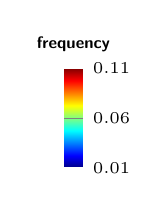
\begin{tikzpicture}
\begin{axis}[font=\bf\sffamily\fontsize{6}{6}\selectfont,
  hide axis,major tick length=0pt,
  xtick=\empty,
    scale only axis,
    height=0pt,
    width=0pt,
    colormap/jet,
    colorbar,
    point meta min=0.01,
    point meta max=0.11,
    colorbar style={title={frequency},title style={yshift=-.05in},font=\bf\sffamily\fontsize{6}{6}\selectfont,draw=none,axis line style={white}, y tick label style={
        /pgf/number format/.cd,
            fixed,
            fixed zerofill,
            precision=2,
        /tikz/.cd
    },  height=.5in,width=.1in,
        ytick={0.01,0.06,0.11}
    }]
    \addplot [draw=none] coordinates {(0,0)};
\end{axis}
\end{tikzpicture}};
  % \node[anchor=north west,label={[]90:{\large b.} 2018-2019 (Northern Hemisphere)}] (T2) at ([xshift=.1in]T1.south west) {
  %   \begin{tikzpicture}[font=\bf\sffamily\fontsize{7}{7}\selectfont]
  %     \node[] (A) at (0,0) {
  %       \mnp{2.65in}{\begin{texshade}{\SEQB}
  %           \shadingmode[chemical]{functional}
  %           \hideallmatchpositions
  %           \rulersteps{1}
  %           \setfont{residues}{sf}{up}{bf}{tiny} 
  %           \setfont{numbering}{sf}{up}{bf}{tiny} 
  %           \setfont{names}{tt}{up}{bf}{small}
  %           \setfont{legend}{tt}{up}{bf}{scriptsize}
  %           \threshold[80]{50}
  %           \setends{1}{1..\LENA}
  %           \showruler{1}{top}
  %           \hideconsensus
  %           \shadeallresidues
  %           \showlegend
  %         \end{texshade}
  %         % 
  %         \begin{texshade}{\SEQB}
  %           %\shadingmode[standard area]{functional}
  %           \shadingmode[hydropathy]{functional}
  %           \hideallmatchpositions
  %           \rulersteps{1}
  %           \setfont{residues}{sf}{up}{bf}{tiny} 
  %           \setfont{numbering}{sf}{up}{bf}{tiny} 
  %           \setfont{names}{tt}{up}{bf}{small}
  %           \setfont{legend}{tt}{up}{bf}{scriptsize}
  %           \threshold[80]{50}
  %           \setends{1}{1..\LENA}
  %           \showruler{1}{top}
  %           \hideconsensus
  %           \shadeallresidues
  %           \showlegend
  %         \end{texshade}
  %         % 
  %         \begin{texshade}{\SEQB}
  %           \shadingmode[accessible area]{functional}
  %           \hideallmatchpositions
  %           \rulersteps{1}
  %           \setfont{residues}{sf}{up}{bf}{tiny}
  %           \setfont{numbering}{sf}{up}{bf}{tiny} 
  %           \setfont{names}{tt}{up}{bf}{small}
  %           \setfont{legend}{tt}{up}{bf}{scriptsize}
  %           \threshold[80]{50}
  %           \setends{1}{1..\LENA}
  %           \showruler{1}{top}
  %           \hideconsensus
  %           \shadeallresidues
  %           \showlegend
  %         \end{texshade}
  %         % 
  %       }};
  %   \end{tikzpicture}};

 %  \node[anchor=north west,label={[]90:{\large c.} 2016-2017 (Southern Hemisphere)}] (T2) at ([xshift=0in]T1.south west) {
%     \begin{tikzpicture}[font=\bf\sffamily\fontsize{7}{7}\selectfont]
%       \node[ ] (A) at (0,0) {
%         \mnp{3.5in}{\begin{texshade}{\SEQC}
%             %\shadingmode[chemical]{functional}
%             \shadingmode[accessible area]{functional}
%             \hideallmatchpositions
%             \rulersteps{1}
%             \setfont{residues}{sf}{up}{bf}{tiny} 
%             \setfont{numbering}{sf}{up}{bf}{tiny} 
%             \setfont{names}{tt}{up}{bf}{small}
%             \setfont{legend}{tt}{up}{bf}{scriptsize}
%             \threshold[80]{50}
%             \setends{1}{1..\LENA}
%             \showruler{1}{top}
%             \hideconsensus
%             \shadeallresidues
%             \showlegend
%           \end{texshade}}};
% \node[] (B) at (A.north east) {  \mnp{3.5in}{      
%           % 
%           \begin{texshade}{\SEQC}
%             %\shadingmode[standard area]{functional}
%             \shadingmode[hydropathy]{functional}
%             \hideallmatchpositions
%             \rulersteps{1}
%             \setfont{residues}{sf}{up}{bf}{tiny} 
%             \setfont{numbering}{sf}{up}{bf}{tiny} 
%             \setfont{names}{tt}{up}{bf}{small}
%             \setfont{legend}{tt}{up}{bf}{scriptsize}
%             \threshold[80]{50}
%             \setends{1}{1..\LENA}
%             \showruler{1}{top}
%             \hideconsensus
%             \shadeallresidues
%             \showlegend
%           \end{texshade}}};


      
%     \end{tikzpicture}};


  

  % \node[anchor=north west,label={[]90:{\large d.} 2016-2017 (Northern Hemisphere)}] (T4) at ([xshift=0in]T3.south west) {
  %   \begin{tikzpicture}[font=\bf\sffamily\fontsize{7}{7}\selectfont]
  %     \node[label={[yshift=-1in,xshift=.15in]170:\mnp{.4in}{\raggedright type \\ \vspace{35pt} sd. chn. area \\ \vspace{35pt} acc. sd. chn.}}] (A) at (0,0) {
  %       \mnp{3.2in}{\begin{texshade}{\SEQD}
  %           \shadingmode[chemical]{functional}
  %           \hideallmatchpositions
  %           \rulersteps{1}
  %           \setfont{residues}{sf}{up}{bf}{tiny} 
  %           \setfont{numbering}{sf}{up}{bf}{tiny} 
  %           \setfont{names}{tt}{up}{bf}{small}
  %           \setfont{legend}{tt}{up}{bf}{scriptsize}
  %           \threshold[80]{50}
  %           \setends{1}{1..\LENA}
  %           \showruler{1}{top}
  %           \hideconsensus
  %           \shadeallresidues
  %           % \showlegend
  %         \end{texshade}
  %         % 
  %         \begin{texshade}{\SEQD}
  %           %\shadingmode[standard area]{functional}
  %           \shadingmode[hydropathy]{functional}
  %           \hideallmatchpositions
  %           \rulersteps{1}
  %           \setfont{residues}{sf}{up}{bf}{tiny} 
  %           \setfont{numbering}{sf}{up}{bf}{tiny} 
  %           \setfont{names}{tt}{up}{bf}{small}
  %           \setfont{legend}{tt}{up}{bf}{scriptsize}
  %           \threshold[80]{50}
  %           \setends{1}{1..\LENA}
  %           \showruler{1}{top}
  %           \hideconsensus
  %           \shadeallresidues
  %           % \showlegend
  %         \end{texshade}
  %         % 
  %         \begin{texshade}{\SEQD}
  %           \shadingmode[accessible area]{functional}
  %           \hideallmatchpositions
  %           \rulersteps{1}
  %           \setfont{residues}{sf}{up}{bf}{tiny}
  %           \setfont{numbering}{sf}{up}{bf}{tiny} 
  %           \setfont{names}{tt}{up}{bf}{small}
  %           \setfont{legend}{tt}{up}{bf}{scriptsize}
  %           \threshold[80]{50}
  %           \setends{1}{1..\LENA}
  %           \showruler{1}{top}
  %           \hideconsensus
  %           \shadeallresidues
  %           % \showlegend
  %         \end{texshade}
  %         % 
  %       }};
  %   \end{tikzpicture}};



  % \node[anchor=north west,label={[]90:{\large e.} 2016-2017 (H3N2 Northern Hemisphere)}] (T5) at ([xshift=0in]T4.south west) {
  %   \begin{tikzpicture}[font=\bf\sffamily\fontsize{7}{7}\selectfont]
  %     \node[label={[yshift=-1in,xshift=.15in]170:\mnp{.4in}{\raggedright type \\ \vspace{35pt} sd. chn. area \\ \vspace{35pt} acc. sd. chn.}}] (A) at (0,0) {
  %       \mnp{3.2in}{\begin{texshade}{\SEQE}
  %           \shadingmode[chemical]{functional}
  %           \hideallmatchpositions
  %           \rulersteps{1}
  %           \setfont{residues}{sf}{up}{bf}{tiny} 
  %           \setfont{numbering}{sf}{up}{bf}{tiny} 
  %           \setfont{names}{tt}{up}{bf}{small}
  %           \setfont{legend}{tt}{up}{bf}{scriptsize}
  %           \threshold[80]{50}
  %           \setends{1}{1..\LENA}
  %           \showruler{1}{top}
  %           \hideconsensus
  %           \shadeallresidues
  %           % \showlegend
  %         \end{texshade}
  %         % 
  %         \begin{texshade}{\SEQE}
  %           %\shadingmode[standard area]{functional}
  %           \shadingmode[hydropathy]{functional}
  %           \hideallmatchpositions
  %           \rulersteps{1}
  %           \setfont{residues}{sf}{up}{bf}{tiny} 
  %           \setfont{numbering}{sf}{up}{bf}{tiny} 
  %           \setfont{names}{tt}{up}{bf}{small}
  %           \setfont{legend}{tt}{up}{bf}{scriptsize}
  %           \threshold[80]{50}
  %           \setends{1}{1..\LENA}
  %           \showruler{1}{top}
  %           \hideconsensus
  %           \shadeallresidues
  %           % \showlegend
  %         \end{texshade}
  %         % 
  %         \begin{texshade}{\SEQE}
  %           \shadingmode[accessible area]{functional}
  %           \hideallmatchpositions
  %           \rulersteps{1}
  %           \setfont{residues}{sf}{up}{bf}{tiny}
  %           \setfont{numbering}{sf}{up}{bf}{tiny} 
  %           \setfont{names}{tt}{up}{bf}{small}
  %           \setfont{legend}{tt}{up}{bf}{scriptsize}
  %           \threshold[80]{50}
  %           \setends{1}{1..\LENA}
  %           \showruler{1}{top}
  %           \hideconsensus
  %           \shadeallresidues
  %           % \showlegend
  %         \end{texshade}
  %         % 
  %       }};
  %   \end{tikzpicture}};


  
\end{tikzpicture}  
  \vspace{0pt}   
  
  \else
  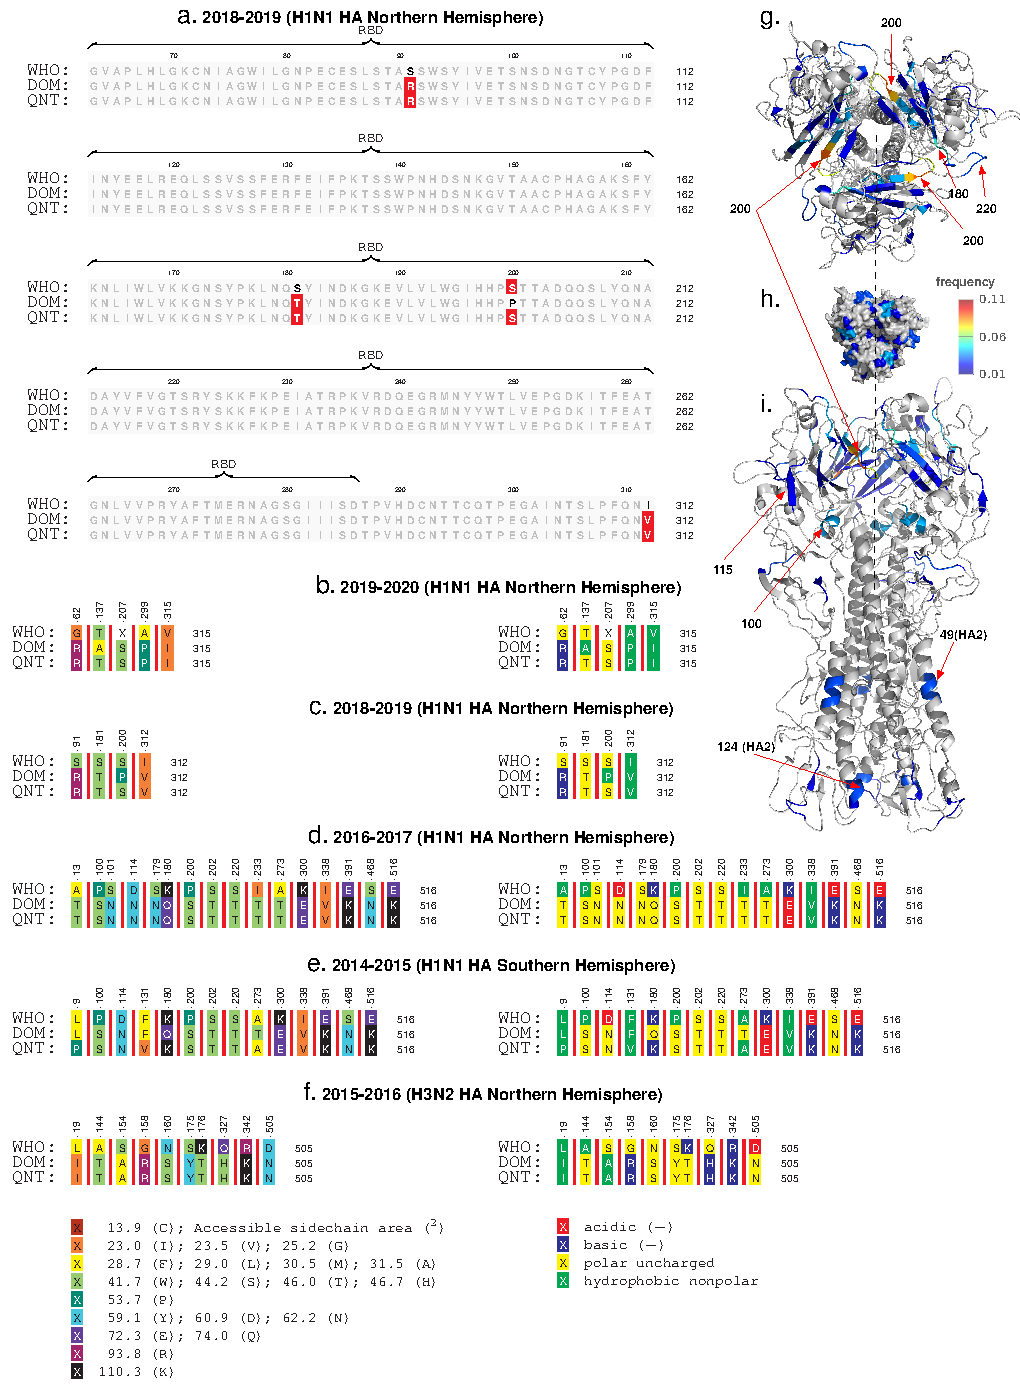
\includegraphics[width=0.87\textwidth]{Figures/External/sequence.pdf}  \vspace{-5pt}   

  \fi
\vspace{0pt}

\captionN{\textbf{Sequence comparisons.} The observed dominant strain, we note that the correct \qnet  deviations tend to be within the RBD, both for H1N1 and H3N2 for HA (panel a shows one example). Additionally, by comparing the type, side chain area, and the accessible side chain area, we note that the changes often have very different properties (panel b-f). Panels g-i show the localization of the deviations in the molecular structure of HA, where we note that the changes are most frequent in the HA1 sub-unit (the globular head), and around residues and structures that have been commonly implicated in receptor binding interactions $e.g$ the $\approx 200$ loop, the $\approx 220$ loop and the $\approx 180$-helix.}\label{figseq}
\end{figure*}
\else
\refstepcounter{figure}\label{figseq}
\fi
%#############################################
%#############################################


%#############################################
%#############################################

\begin{table}\centering
\captionN{Riskiest Strains Currently Circulating in Swine}\label{tabrec11}

\sffamily\fontsize{7}{8}\selectfont

\begin{tabular}{L{2.1in}|L{0.7in}|L{0.7in}|L{0.7in}}\hline
 \rowcolor{lightgray}H1N1 Strain & HA Risk & NA Risk & Overall Risk \\\hline
 A/swine/Tennessee/A02524414/2022 &0.0201&0.0030&0.0077\\\hline
 A/swine/Missouri/A02750646/2022 &0.0201&0.0070&0.0118\\\hline
 A/swine/Kansas/A02711847/2022 &0.0201&0.0098&0.0141\\\hline
 A/swine/Iowa/A02636572/2022 &0.0166&0.0225&0.0193\\\hline
 A/swine/Iowa/A02636308/2021 &0.0143&0.0266&0.0195\\\hline
 A/swine/Illinois/A02750711/2022 &0.0166&0.0233&0.0197\\\hline
 A/swine/Iowa/A02636616/2022 &0.0166&0.0233&0.0197\\\hline
 A/swine/Oklahoma/A02246915/2022 &0.0166&0.0233&0.0197\\\hline
 A/swine/Colorado/A02636469/2022 &0.0166&0.0233&0.0197\\\hline
 A/swine/Iowa/A02636297/2021 &0.0149&0.0267&0.0200\\\hline
 \rowcolor{lightgray}H3N2 Strain & HA Risk & NA Risk & Overall Risk \\\hline
 A/swine/Indiana/A02636492/2022 &0.0104&0.0113&0.0108\\\hline
 A/swine/Indiana/A02636512/2022 &0.0104&0.0113&0.0108\\\hline
 A/swine/Iowa/A02750695/2022 &0.0110&0.0120&0.0115\\\hline
 A/swine/Oklahoma/A02711859/2022 &0.0122&0.0114&0.0118\\\hline
 A/swine/Iowa/A02636351/2022 &0.0121&0.0119&0.0120\\\hline
 A/swine/Iowa/A02636476/2022 &0.0121&0.0120&0.0121\\\hline
 A/swine/Texas/A02636569/2022 &0.0122&0.0120&0.0121\\\hline
 A/swine/Iowa/A02750726/2022 &0.0123&0.0120&0.0121\\\hline
 A/swine/Iowa/A02750740/2022 &0.0104&0.0156&0.0127\\\hline
 A/swine/Indiana/A02636521/2022 &0.0104&0.0156&0.0127\\\hline
 \end{tabular}
\flushleft

\fontsize{7}{7}\selectfont
$^\star$ Converted IRAT Score computed using regression generated from the IRAT vs. Qnet comparison
\end{table}
%#############################################
%#############################################







\clearpage
empty


\clearpage



{\color{magenta}

  

{\color{Red1}
  \section*{Discussion}
  In the aftermath of the COVID-19 pandemic that caused one of the most devastating disasters of the past century, a looming question is whether we can prepare for, preempt and mitigate such events in the future. Evolving viruses, whether currently circulating in the human population, or in animal reservoirs that might spillover and attain human-to-human transmission capability, pose an ever-present epidemic risk.  Current surveillance paradigms, while crucial for mapping disease ecosystems, are limited in their ability to address this challenge. Habitat encroachment, climate change, and other ecological factors~\cite{rulli2017nexus,chua2002anthropogenic,childs2004zoonotic} unquestionably drive up the odds of zoonotic spill-overs. Nevertheless, current efforts at tracking these effects have not improved our ability to quantify future risk of emergence~\cite{fair2019viral}. Tracking viral diversity in animal hosts, while important, often does not transparently map to emergence risk.  This is particularly true for \infl, which partly on account of its segmented genome, can easily incorporate genes from multiple strains and emerge as novel human pathogens, and thus harbor a high pandemic potential. While large antigenic shifts in \infl are relatively rare, even the smaller seasonal sequence alterations in cause sufficient variation in the surface proteins to evade existing immunity, and require yearly reformulation of the flu vaccine.

  However, for the  vaccine to be effective, we need to  predict the dominant circulating strain of the upcoming season with sufficient accuracy.
  Currently, the composition of the flu shot is decided at least six months in advance of the seasonal infection peak, and targets three to four  historical strains as recommended by the CDC/WHO, who identify these specific strains by  sampling the current circulation~\cite{agor2018models}, hoping to match the  dominant strain(s) in the upcoming season. A variety of hard-to-model effects hinder this prediction, which, despite observed cross-reactive effects~\cite{tricco2013comparing}, have had  limited vaccine effectiveness in recent years~\cite{cdceff}. Rank-ordering strains which do not yet circulate in humans according to either their spillover risk or their pandemic potential, has proven to be even more difficult [REF]. CDC's current, somewhat subjective, solution to this problem is the Influenza Risk Assessment Tool (IRAT), which  uses a combination of ten weighted risk elements, including  1) properties of the virus, 2) attributes of the population, and 3) ecology and epidemiological characteristics of the virus~\cite{Influenz24:online} that are expert-selected. Evaluating these factors involve several experimental assay for each strain, taking possibly weeks to return the final IRAT  score for a single strain. Thus, we have a scalability problem: with  the current global biosurveillance efforts  collecting tens of thousands of sequences every year, IRAT assessment is simply not fast enough to  preempt a pandemic. }



\section*{Discussion \& Sequence Comparisons}

For further discussion, we looked at our \qnet predictions more closely. Comparing the \qnet inferred strain (QNT) against the one recommended by the WHO, we find: 1) the residues that only the QNT matches correctly with DOM (while the WHO fails) are largely localized within the receptor binding domain (RBD), with $>57\%$ occurring within  the RBD on average (see Fig.~\ref{figseq}a for a specific example), and 2) when the WHO strain deviates from  the QNT/DOM  matched residue, the ``correct'' residue is often replaced in the WHO recommendation with one that has very different side chain, hydropathy  and/or chemical properties (see Fig.~\ref{figseq}b-f), suggesting deviations in recognition characteristics. Combined with the fact that we find circulating strains are almost always within a few edits of the DOM (see SI-Fig.~\ref{SI-figdom}), these observations suggest that hosts vaccinated with the QNT recommendation is more likely to have season-specific antibodies that are more likely to recognize a larger cross-section of the circulating strains.

High season-to-season genomic variation in the key  Influenza capsidic proteins is driven by two opposing influences: 1) the need to conserve function  limiting random mutations, and 2) hyper-variability to escape recognition by neutralizing antibodies. Even a  single residue change in the surface proteins might dramatically alter recognition characteristics, brought about by unpredictable~\cite{carugo2001normalized,righetto2014comparative} changes in local or regional properties such as charge, hydropathy, side chain solvent accessibility~\cite{lee1971interpretation,shrake1973environment,momen2008impact,adamczak2005combining}.

Focusing on the average localization of the QNT to WHO deviations in the HA molecular  structure, the changes are observed to primarily occur in the HA1 sub-unit (see Fig.~\ref{figseq}g-i, HA0 numbering used, other numbering conversions are given in SI-Table~\ref{SI-tabnum}), with the most frequent deviations  occurring around the $\approx 200$ loop, the $\approx 220$ loop, the $\approx 180$ helix, and the $\approx 100$ helix, in addition to some residues in the HA2 sub-unit ($\approx 49$ \& $\approx 124$). Unsurprisingly, the residues we find to be most impacted in the HA1 sub-unit (the globular top of the fusion protein) have been repeatedly implicated in receptor binding interactions~\cite{tzarum2015structure,lazniewski2018structural,garcia2015dynamic}. Thus, we are able to fine tune the future recommendation over the state of the art, largely by modifying residue recommendations around the RBD and  structures affecting recognition dynamics.



}

{\color{Green1}


  It is well known that the influenza viral RNA-polymerase represents the lack of proofreading function. Thus, the integration of faulty nucleotides often occurs during the viral replication process with a rate of $10^{-3}$ to $10^{-4}$, which results in high mutation rates [39,40].



  
  Due to its crucial role in receptor recognition and attachment, IAV HA is considered to be a principal determinant of the host-range. The specificity of the HA of avian influenza viruses is for $\alpha-2,3$ SA receptors found in the intestinal tract of the bird, whereas $\alpha-2,6$ SA receptors are predominantly found in the upper respiratory tract of humans. Recently, it has been shown that mutations in the HA protein alter its receptor-binding preference that allows the highly pathogenic avian H5N1 IAV to transmit between mammals [41]. Therefore, it is not surprising that multiple changes in gene segments of the avian influenza virus could result in its adaptation to humans [1]. On the other hand, owing to having both $\alpha-2,3$ and $\alpha-2,6$  linkages, pigs and several avian species (pheasants, turkeys, quails) may act as mixing vessels and can generate re-assortment viruses [42,43].


  Influenza proteins must evade immune recognition while maintaining their ability to function and interact with host cellular factors [44]. The three mechanisms by which influenza viruses undergo evolutionary change include mutation (antigenic drift), re-assortment (antigenic shift), and, in rare instances, recombination. The different virus lineages are predominantly host specific, but there are periodic exchanges of influenza virus gene segments between species, giving rise to pandemics of disease in humans, lower animals, and birds [45]. Influenza virus evolution proceeds via re-assortment and mutation, and such evolution can influence the host specificity and pathogenicity of these viruses [46]. Genetic variations of influenza A virus lead to possible changes in upcoming epidemiological behavior and may result in human pandemics.


  Significant mutations in antigenic sites resulting from constant point mutations in the influenza virus contribute to the gradual evolution of the virus, leading to antigen migration to produce new influenza virus subtypes to escape the immune pressure of the population [47]. All subtypes of influenza A virus antigenic drift can occur, but such antigenic drift often occurs in the general human influenza. Immune escape can be achieved by mutation in IAV proteins such as HA and/or NA. The minimal structural changes can occur in these surface proteins and so the immune protection of the host (acquired through previous infections or immunization) will no longer be effective against the invading virus. As a consequence, the immune system is unable to identify the newly changed virus variants and the recognition pattern of the antigen-antibody-interaction is not fully functional anymore. In addition, amino acid substitutions in HA protein can change the receptor preference of influenza virus. Some studies have shown that the G186V mutation in HA protein was noted as a potential adaptation of avian H7 to human-type receptors [48,49]. In A/Vietnam/1203/2004 (H5N1) virus, K58I substitution in HA protein is associated with increased viral replication of upper respiratory tracts in mice and ferrets [50]. Remarkably, the K58I substitution combined with a G219S mutation in HA protein increased the overall affinities of binding to  $\alpha-2,3$ and  $\alpha-2,6$ SA of the A/Anhui/1/13 (H7N9) virus [51]. Furthermore, there is a R292K mutation in NA protein in H7N9 virus strains which had been isolated from a patient after drug treatment. This substitution was found to promote drug resistance; in particular, it gave a high resistance to oseltamivir which is the most commonly used anti-influenza drug [52]. Antigenic drifts are the main reason for new variants and cause annual influenza outbreaks. Although these changes may not lead to pandemics, antigenic drift over a period of time can make a strain considerably different from the original pandemic virus.

  It has been confirmed that the long-term evolution of cytotoxic T lymphocyte (CTL) epitopes is associated with CTL-mediated clearance of infection and it is thought that the selection pressures imposed by CTL immunity shape the long-term evolution of IAV [53,54]. Viruses mutate amino acid residues within CTL epitopes to evade CTL recognition [55]. Under certain circumstances, amino acid substitutions occur at the anchoring residues, while in other cases they occur at the T cell receptor contact residues [56]. For instance, mutations at the anchored residues of the CTL epitope have been described in the human leukocyte antigen (HLA)-B* 2705 restricted NP383–391 epitope, which has the R-to-G substitution at position 384 (R384G) [57,58]. This replacement significantly reduced the in vitro virus-specific CTL response in HLA-B* 2705-positive individuals.

  4.2. Re-Assortment
  It has been well recognized that the segmented genome of the influenza virus allows the exchange of RNA segments between genotypically different influenza viruses, resulting in the production of new strains and/or subtypes [67], which is referred to as re-assortment. A pandemic IAV can be produced by transmission from animals to humans or by reconfiguration between avian influenza viruses and human influenza viruses [68]. As the influenza virus has a segmented genome, re-assortment is an important mechanism for generation of the "novel" virus [69]. Thus, re-assortment of the virus achieves a new antigenic pattern known as "antigenic shift". Pandemic influenza emerges as a result of such major genetic changes of IAV. These modifications occur due to mechanistic errors during the replication of viral RNA polymerase, evolutionary pressure, the novel environment of the host, immune pressure, or antiviral drug pressure [70]. Two of the three major human influenza pandemics in the twentieth century (1957 and 1968) and this century (2009) were due to the re-assortment between the human IAV and other host species.


  There is evidence indicating that the HA, NA, and PB1 genes of the H2N2 1957 pandemic strain in addition to the HA and PB1 fragments of the H3N2 1968 pandemic strain are both avian, and the remaining fragments may come directly from 1918 [67]. The first influenza pandemic in this century, the influenza A H1N1 virus, is a re-assortant caused by a multiple mixed recombination between the European H1N1 swine influenza virus, North American H1N2 swine influenza virus, North American avian influenza virus, and H3N2 influenza virus [71].

  In addition to mutation and re-assortment, IAVs still have another relatively rare means of evolution called recombination. Genetic recombination is one of the primary processes that produce the genetic diversity upon which natural selection acts. Recombination in IAVs can occur through two main mechanisms: one is the non-homologous recombination that occurs between two different RNA fragments [81,82]; the other is the controversial homologous recombination, often considered to be absent or very rare, which is thought to participate in template switching while the polymerase is copying the RNA.



  Wild waterfowl and shorebirds belong to the main natural host species of IAV [88]. IAV has been able to establish the successful infection of a variety of animals, including avian and mammalian species, and its evolution has led to the emergence of IAV in human beings for a long time [89]. Since the pandemic outbreak of influenza virus in 1918, the re-assortment of influenza virus has occurred among bird and human viruses. As described above, the re-assortment of influenza viruses has resulted in the pandemic of H2N2 in 1957 and of H3N2 in 1968 [90]. During the year 2009, there was an outbreak of H1N1 in humans that caused the first pandemic of influenza through human transmission in the 21st century [91].

  Usually, an avian influenza subtype does not infect humans and a human influenza subtype is unable to infect the birds. However, swine acts as a virus mixer vessel, leading to the generation of new influenza viruses, which can infect both humans and poultry. The mutation and re-assortment of the IAV genome are susceptible to forming new subtypes of influenza virus that may result in widely propagated and destructive pandemics due to the lack of immunity to the emerging pathogen [67]. For example, the outbreak of H5N1 avian influenza in 1997 and the outbreak of H1N1 swine influenza in 2009 caused great panic and brought serious economic losses to the breeding industry.



}


\section*{Brief Methods}
\DQS{review more craefully phenotypic info used in teh literature and why it is claimed to be necessary in those papers. Why dont we need it}
A key barrier to making progress  on both the problems cited above, namely predicting the dominant strain(s) in seasonal flu, as well as estimating the numerical odds of an animal strain  to spillover and attain HH capability,  is our limited understanding of the emergent dependencies across individual mutations that  constrain evolutionary trajectories. Thus, to the best of our knowledge, the state of the art has no tools to estimate the numerical likelihood of specific mutations in the future, and in general  the likelihood of a wild strain spontaneously giving rise to another by random chance. Currently, this likelihood is often qualitatively equated to sequence similarity, which is measured by the number of mutations it takes to change one strain to another. However, the odds of one sequence mutating to another is not just a function of how many mutations separate them, but also of how specific mutations incrementally affect fitness. Ignoring the constraints arising from the need to conserve function makes any assessment of the mutation likelihood open to subjective bias. Here, we show that a precise calculation is possible when sequence similarity is evaluated via a new biologically-aware metric, which we call the \textit{q-distance}.

Some recent efforts have recognized this gap, and have attempted to predict future dominant strain by incorporating other phenotypic details. 

As an applications of the q-distance, we show that we can improve seasonal forecasts for the future dominant circulating strain by learning from the mutational patterns of key surface proteins: Hemaglutinnin (HA) and Neuraminidase (NA) for Influenza A. We outperform the WHO's recommendations for the flu-shot composition consistently over past two decades, measured as the number of mutations that separate the predicted from the dominant circulating strain in each season. Our recommendations repeatedly end up closer to the dominant circulating strain, illustrating the potential of our approach to correctly predict evolutionary trajectories. 

We also show that this new metric allows us to  assess the risk posed by novel strains  effectively and quickly. We compare q-distance results to the CDC's Influenza Risk Assessment Tool (IRAT)~\cite{Influenz24:online}, which gives a grade between 1-10 for emergence risk and public health impact to Influenza A viruses not currently circulating among humans. Our results show strong negative correlations between IRAT emergence risk grades and q-distances to the nearest human strains to the strains in question. However, while IRAT may take weeks to analyze a single strain -- hence the small number of analyzed strains -- q-analysis can be done within milliseconds for each new strain. Moreover, q-analysis only requires sequence data, while IRAT requires information for 10 risk elements, grouped into three categories: 1) properties of the virus, 2) attributes of the population, and 3) ecology and epidemiology of the virus~\cite{Influenz24:online}. Thus, our method could potentially be a low-cost, efficient substitute to IRAT, which could used at scale to rank the risk of emergence of non-circulating strains.

{\color{Red1} Discussion? 
  Thus, the tool proposed in this study  can  profoundly impact  bio-surveillance strategies. The ability to rank newly collected strains by risk at scale, allows actionable estimates of  pandemic risks via  quantifying the odds of a particular strain spilling into to the human population. Additionally,  for strains already circulating in humans, our tools can estimate the odds  of specific  new mutan varaints emerging, and their ability to  escape current vaccines. %This study potentially represents an important step forward in modeling emerging pathogens, with uncharted impact on science and health, particularly as we prepare for the aftermath of \cov.
}

\end{document}
% LocalWords:  Neuraminidase subtype
